\documentclass[letterpaper, 12pt]{article}
% \usepackage[showframe, margin=1in, top=0.25in, bottom=0.25in, includeheadfoot, headheight=0.5in]{geometry}
\usepackage[margin=1in, top=0.25in, bottom=0.25in, includeheadfoot, headheight=0.5in]{geometry}

\AddToHook{cmd/section/before}{\clearpage}

\usepackage[table]{xcolor}
\colorlet{listingback}{gray!20}
\definecolor{headingcolor}{RGB}{110,34,54}

\usepackage{fancyhdr}
\renewcommand{\sectionmark}[1]{\markboth{#1}{#1}}

% Used to detect whether a section is an appendix to print the right thing in the footer
\usepackage{etoolbox}
\newtoggle{inappendix}
\pretocmd{\appendix}{\clearpage\toggletrue{inappendix}}{}{}

% Save standard definitions for head and foot rules (lines separating header and footer from text)
\let\HeadRule\headrule
\let\FootRule\footrule
% Add color to the standard definitions
\renewcommand{\headrule}{\color{headingcolor}\HeadRule}
\renewcommand{\footrule}{\textcolor{headingcolor}{\FootRule}}

% IMPORTANT: This command should not be called directly. Use \preamble.
% Macro to insert the title page for each lab.
% The argument is the title of the lab.
\newcommand{\inserttitlepage}[1]
{
    \begin{titlepage}
    \centering
    
\includegraphics[scale=0.5]{images/nexus_lab_logo.png}

    \vspace*{\baselineskip}

    \textbf{\Large OpenStack Labs}

    \vspace*{\baselineskip}

    \textbf{\Large #1}
    \vspace*{\fill}
\end{titlepage}
}

% IMPORTANT: This command should not be called directly. Use \preamble.
% Macro to define header and footer for each lab.
% The argument is the title of the lab.
\newcommand{\headfoot}[1]
{
    \fancypagestyle{fancy}
    {
        \fancyhf{}
        \fancyhead[L]{\footnotesize #1}
        \fancyhead[R]{
\includegraphics[height=0.85\headheight]{images/nexus_lab_logo.png}}
        \fancyfoot[L]{%
            \footnotesize%
            \ifnum\value{section}>0%
            \iftoggle{inappendix}{Appendix \thesection: \rightmark}{Section \thesection: \rightmark}%
            \fi}
        \fancyfoot[R]{\footnotesize\thepage}
        \renewcommand{\headrulewidth}{1.5pt}
        \renewcommand{\footrulewidth}{1.5pt}
    }
}

% Macro to insert title page, define header and footer, and insert table of contents and about section for each lab.
% The argument is the title of the lab.
\newcommand{\preamble}[1]
{
    \pagenumbering{roman}
    \inserttitlepage{#1}
    \headfoot{#1}

    % Insert table of contents
    \pagestyle{fancy}
    \tableofcontents
    \clearpage

    \section*{About This Document}
    \label{sec:about_this_document}
    \begin{itemize}
        \item This document was developed by a team at the University of Tennessee at Chattanooga led by Dr. Mengjun Xie
        (\href{mailto:mengjun-xie@utc.edu}{\textbf{mengjun-xie@utc.edu}}).
        \item The development of this document was supported by a National Centers of Academic Excellence in Cybersecurity Grant (\#H98230-20-1-0351), housed at the National Security Agency.
        \item This document is licensed with a Creative Commons Attribution 4.0 International License.
    \end{itemize}
    \clearpage
}

% Macro to insert the Lab Settings page for each lab. Call after the Introduction and Objectives sections.
\newcommand{\labsettings}
{
    \section*{Lab Settings}
    \label{sec:lab_settings}
    \addcontentsline{toc}{section}{\nameref{sec:lab_settings}}
    The information in the table below will be needed in order to complete the lab.
    The task sections below provide details on the use of this information.
    \begin{table*}[htbp]
        \centering
        \begin{tabular}{|c|c|c|c|}
            \hline
            \rowcolor{gray!20} \textbf{Virtual Machine} & \textbf{IP Address} & \textbf{Account} & \textbf{Password} \\
            \hline
            \multirow{2}{*}{\texttt{workstation}} & \multirow[t]{2}{*}{\texttt{ens3: 192.168.1.21}}  & \multirow{2}{*}{\texttt{ubuntu}} & \multirow{2}{*}{\texttt{ubuntu}} \\
                                                  & \multirow[t]{2}{*}{\texttt{ens4: 172.25.250.21}} &                                  &                                  \\
            \hline
            \multirow{2}{*}{\texttt{devstack}}    & \multirow[t]{2}{*}{\texttt{ens3: 192.168.20}}    & \multirow{2}{*}{\texttt{ubuntu}} & \multirow{2}{*}{\texttt{ubuntu}} \\
                                                  & \multirow[t]{2}{*}{\texttt{ens4: 172.25.250.20}} &                                  &                                  \\
            \hline
        \end{tabular}
    \end{table*}
    \clearpage

    % IMPORTANT(lucas): If another frontmatter section ever gets placed after this, this command needs to be moved
    % to the end of that section.
    % I have placed this here and not in each lab purely for convenience and to ensure I don't forget any.
    \pagenumbering{arabic}
}

% Sans-serif font
\renewcommand{\familydefault}{\sfdefault}
\newcommand{\texttildemid}{{\raisebox{0.5ex}{\texttildelow}}}

\usepackage{enumitem}
\renewcommand{\labelenumi}{\textbf{\thesection.\arabic{enumi}.}}

% Try to forbid widows and orphans
\widowpenalty10000
\clubpenalty10000

\usepackage{graphicx}
\usepackage{hyperref}
\hypersetup{colorlinks=true,linkcolor=black,urlcolor={[named] headingcolor}}

\usepackage{sectsty}
\sectionfont{\color{headingcolor}}

% Table of Contents
\usepackage{bookmark}
\usepackage[titles]{tocloft}
\usepackage[title]{appendix}
\renewcommand{\cfttoctitlefont}{\Large\bfseries\color{headingcolor}}
\renewcommand{\cftsecfont}{\normalfont\normalsize}
\renewcommand{\cftsecpagefont}{\normalfont\normalsize}
\renewcommand{\cftdotsep}{0} % Make dots small and close together
\renewcommand{\cftsecleader}{\cftdotfill{\cftdotsep}} % Add dots after section titles
% Make dots go all the way to the page number
\renewcommand{\cftsecfillnum}[1]{{\cftsecleader}\nobreak{\cftsecpagefont #1}\cftsecafterpnum\par}

\usepackage{multirow}
\setlength{\tabcolsep}{16pt}
\renewcommand{\arraystretch}{1.1}

% For nice-looking boxes
\usepackage[most]{tcolorbox}
\usepackage{listings}
\usepackage{lstautogobble}
\lstset{
  frame=none,
  language=Bash,
  showstringspaces=false,
  basicstyle={\linespread{1.1}\footnotesize\ttfamily\selectfont},
  numbers=none,
  breaklines=true,
  breakatwhitespace=true,
  tabsize=3,
  columns=fullflexible,
  keepspaces=true,
  escapeinside={(*@}{@*)},
  literate={~}{{\texttildemid}}{1}
           {\#}{\#}{1},
  autogobble=true
}

\tcolorboxenvironment{lstlisting}
{
    spartan,
    colframe=gray!50,
    boxsep=0mm,
    left=1mm,
    right=1mm,
    top=-1mm,
    bottom=-1mm,
    colback=gray!20
}

% Hacky solution for now, would like to have just one environment and make several tcolorboxes by passing different
% colors as parameters, but that is giving errors
\makeatletter
\tcbset{
  note/.style={%
        enhanced,
        breakable,
        colback=blue!10!white,
        colframe=blue!80!white,
        attach boxed title to top left={yshift*=-\tcboxedtitleheight},
        title={#1},
        boxed title size=title,
        boxed title style={%
            sharp corners,
            rounded corners=northwest,
            colback=tcbcolframe,
            boxrule=0pt,
        },
        underlay boxed title={%
            \path[fill=tcbcolframe] (title.south west)--(title.south east)
                to[out=0, in=180] ([xshift=5mm]title.east)--
                (title.center-|frame.east)
                [rounded corners=\kvtcb@arc] |-
                (frame.north) -| cycle;
        },
    }
}
\makeatother

\makeatletter
\tcbset{
    stop/.style={%
        enhanced,
        breakable,
        colback=white,
        colback=red!10!white,
        colframe=red!80!white,
        attach boxed title to top left={yshift*=-\tcboxedtitleheight},
        title={#1},
        boxed title size=title,
        boxed title style={%
            sharp corners,
            rounded corners=northwest,
            colback=tcbcolframe,
            boxrule=0pt,
        },
        underlay boxed title={%
            \path[fill=tcbcolframe] (title.south west)--(title.south east)
                to[out=0, in=180] ([xshift=5mm]title.east)--
                (title.center-|frame.east)
                [rounded corners=\kvtcb@arc] |-
                (frame.north) -| cycle;
        },
    }
}
\makeatother

\makeatletter
\tcbset{
    tip/.style={%
        enhanced,
        breakable,
        colback=white,
        colback=green!10,
        colframe=green!70!black,
        attach boxed title to top left={yshift*=-\tcboxedtitleheight},
        fonttitle=\bfseries,
        title={#1},
        boxed title size=title,
        boxed title style={%
            sharp corners,
            rounded corners=northwest,
            colback=tcbcolframe,
            boxrule=0pt,
        },
        underlay boxed title={%
            \path[fill=tcbcolframe] (title.south west)--(title.south east)
                to[out=0, in=180] ([xshift=5mm]title.east)--
                (title.center-|frame.east)
                [rounded corners=\kvtcb@arc] |-
                (frame.north) -| cycle;
        },
    }
}
\makeatother

% The commands below define environments for colored boxes. They are used like
% \begin{notebox}
% ...
% \end{notebox}
\newtcolorbox{notebox}{note={Note}}
\newtcolorbox{stopbox}{stop={Stop}}
\newtcolorbox{tipbox}{tip={Tip}}

\begin{document}
\preamble{Lab 06: Managing an OpenStack Instance}

\section*{Introduction}\label{sec:introduction}
\addcontentsline{toc}{section}{\nameref{sec:introduction}}
Up to this point, whenever you have launched an instance, its resources and running state have remained mostly constant.
However, OpenStack instances are quite flexible, even after being launched.
In this lab, you will launch an instance and perform several management operations while it is running.

\section*{Objectives}\label{sec:objectives}
\addcontentsline{toc}{section}{\nameref{sec:objectives}}
\begin{itemize}[itemsep=0pt]
    \item Create a snapshot of an instance.
    \item Manage the running and power state of an instance.
\end{itemize}
\clearpage

\labsettings

%%%%%%%%%%%
% Section 1
%%%%%%%%%%%
\section{Creating a Snapshot with the Horizon Dashboard}\label{sec:creating_a_snapshot_web}
In this task, you will launch an instance, modify its configuration, and make a snapshot of it for later use.
Taking a snapshot of an image captures its state and data on disk.
An OpenStack snapshot can be used as an image to launch other instances.
There are a couple situations where snapshots might be a useful tool.
One is to aid in the backup of instance or as a precaution before a major change so that the image is easily recoverable.
Another use of snapshots is to build off an existing image to create a better template for new instances.
For instance, consider the case where you want to launch multiple customized FTP servers.
Instead of launching each one from a basic Ubuntu image and modifying their configurations individually, you might set up one instance completely and take a snapshot.
That snapshot could then be used as a template for the other instances to save time and prevent mistakes.

\begin{enumerate}
    \begin{labstep}
        Log into the \textbf{workstation} machine as the \textbf{ubuntu} user with password \textbf{ubuntu}.

        \begin{center}
            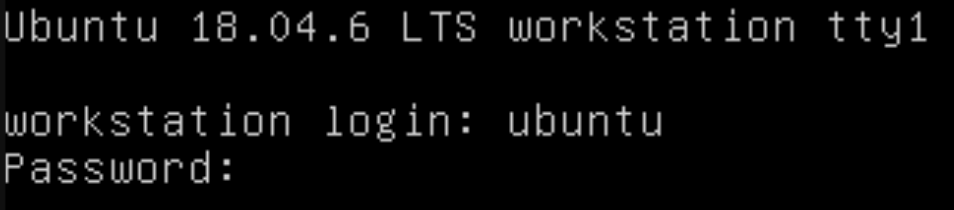
\includegraphics[width=\linewidth]{images/part1/step1.png}
        \end{center}
    \end{labstep}

    \begin{labstep}
        Launch the graphical user interface.
        \begin{lstlisting}
            ubuntu@workstation:~$ startx
        \end{lstlisting}

        \begin{center}
            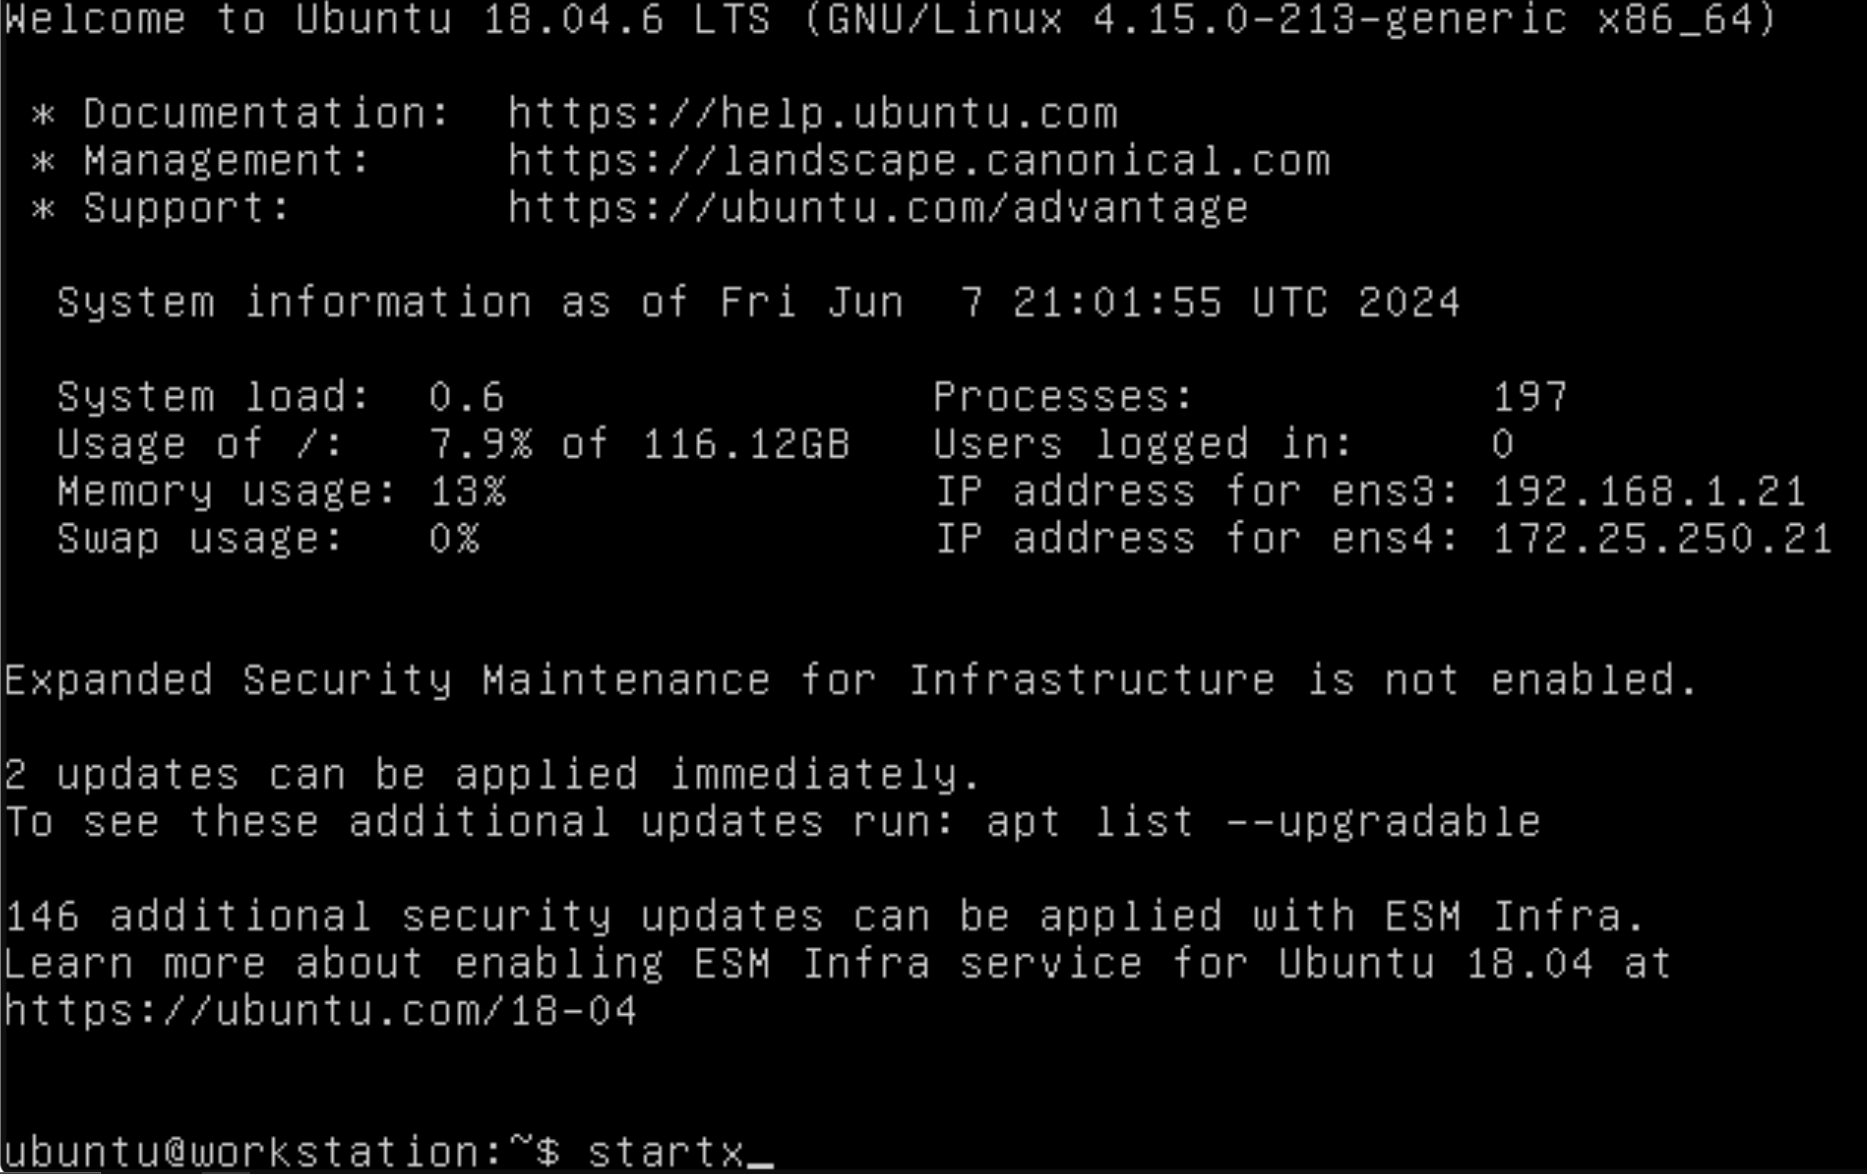
\includegraphics[width=\linewidth]{images/part1/step2.png}
        \end{center}
    \end{labstep}

    \begin{labstep}
        Open the web browser and navigate to \textbf{192.168.1.20}.
        Log into the dashboard as \textbf{admin} with the password \textbf{secret}.
    \end{labstep}

    \begin{labstep}
        Ensure the \textbf{demo} project is selected.
        Navigate to \textbf{Project $>$ Compute $>$ Instances}, and click \textbf{Launch Instance}.

        \begin{center}
            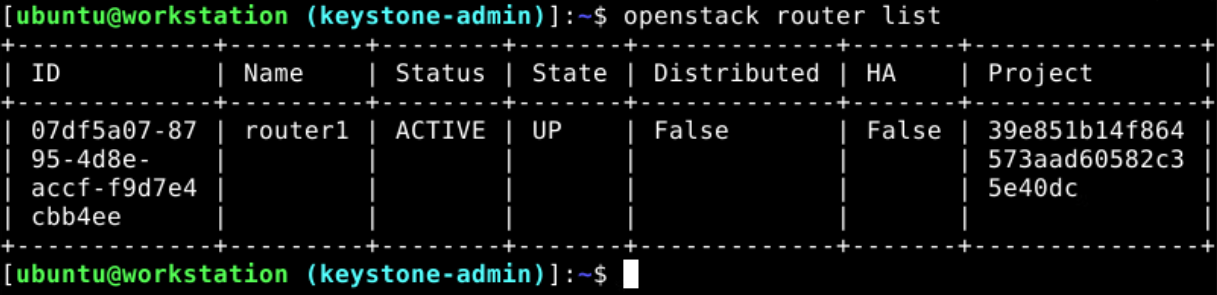
\includegraphics[width=\linewidth]{images/part1/step4.png}
        \end{center}
    \end{labstep}

    \begin{labstep}
        In the \textit{Details} tab, enter \textbf{instance1} in the \textit{Instance Name} field and click \textbf{Next}.

        \begin{center}
            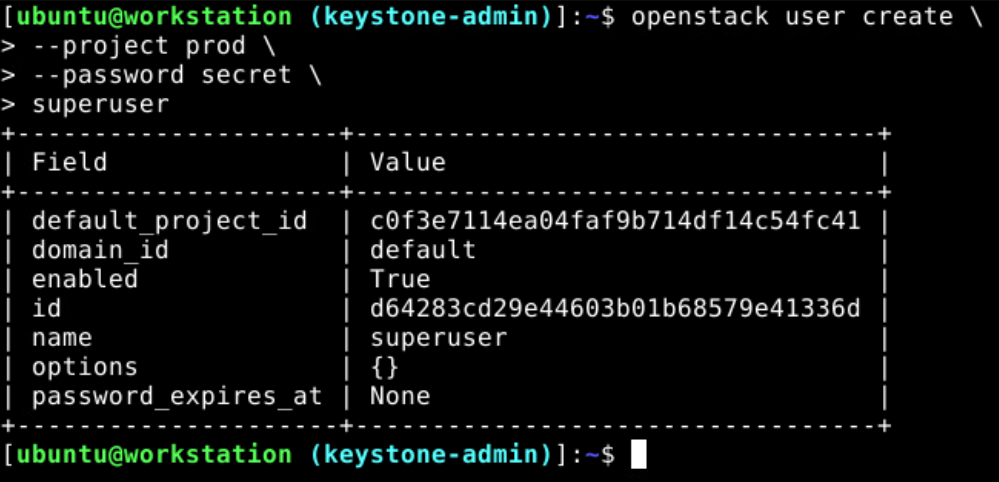
\includegraphics[width=\linewidth]{images/part1/step5.png}
        \end{center}
    \end{labstep}

    \begin{labstep}
        In the \textit{Source} tab, make sure \textbf{Image} is selected in the \textit{Select Boot Source} dropdown and select \textbf{No} under \textit{Create New Volume}.
        Select the \textbf{ubuntu} image by clicking the $\uparrow$ symbol in the same row.
        Click \textbf{Next}.

        \begin{center}
            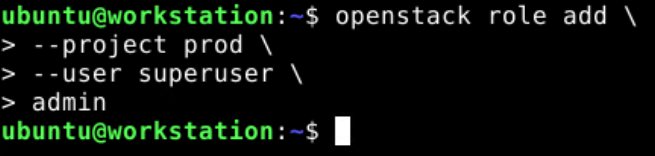
\includegraphics[width=\linewidth]{images/part1/step6.png}
        \end{center}
    \end{labstep}

    \begin{stopbox}
        Before proceeding to the next step, confirm that \textbf{ubuntu} appears underneath the \textit{Allocated} section.
    \end{stopbox}

    \begin{labstep}
        In the \textit{Flavor} tab, click the $\uparrow$ symbol in the same row as \textbf{m1.small}.
        Click \textbf{Next}.

        \begin{center}
            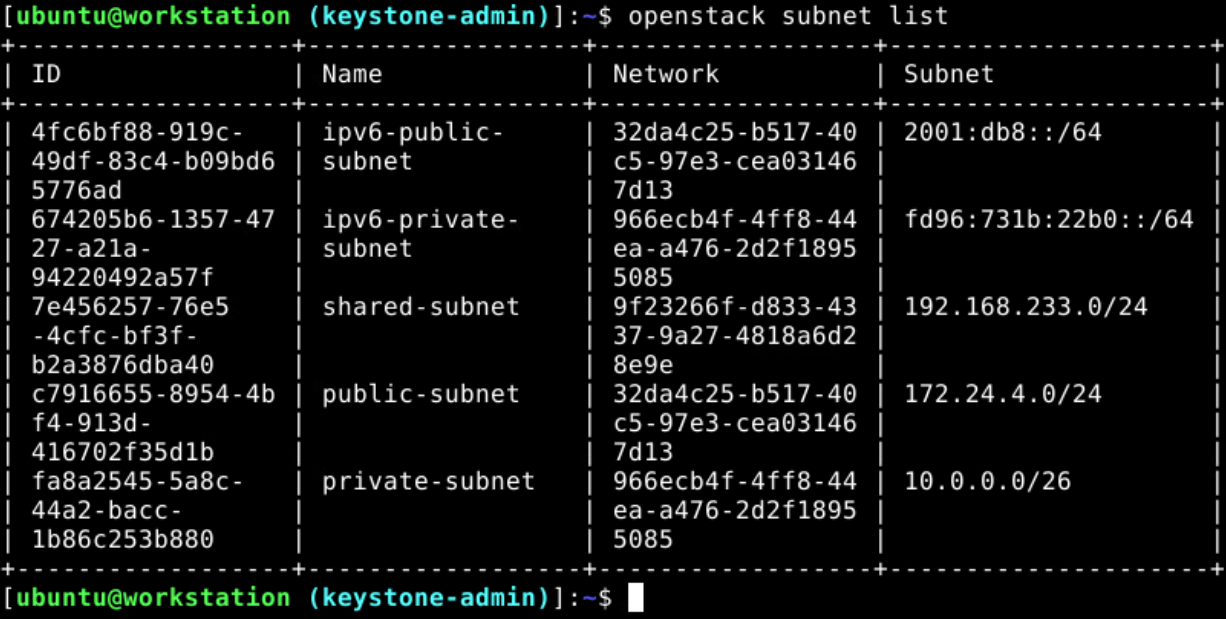
\includegraphics[width=\linewidth]{images/part1/step7.png}
        \end{center}
    \end{labstep}

    \begin{stopbox}
        Before proceeding to the next step, confirm that \textbf{m1.small} appears underneath the \textit{Allocated} section.
    \end{stopbox}

    \begin{labstep}
        In the \textit{Networks} tab, click the $\uparrow$ symbol in the same row as \textbf{shared}.
        Click \textbf{Launch Instance}.

        \begin{center}
            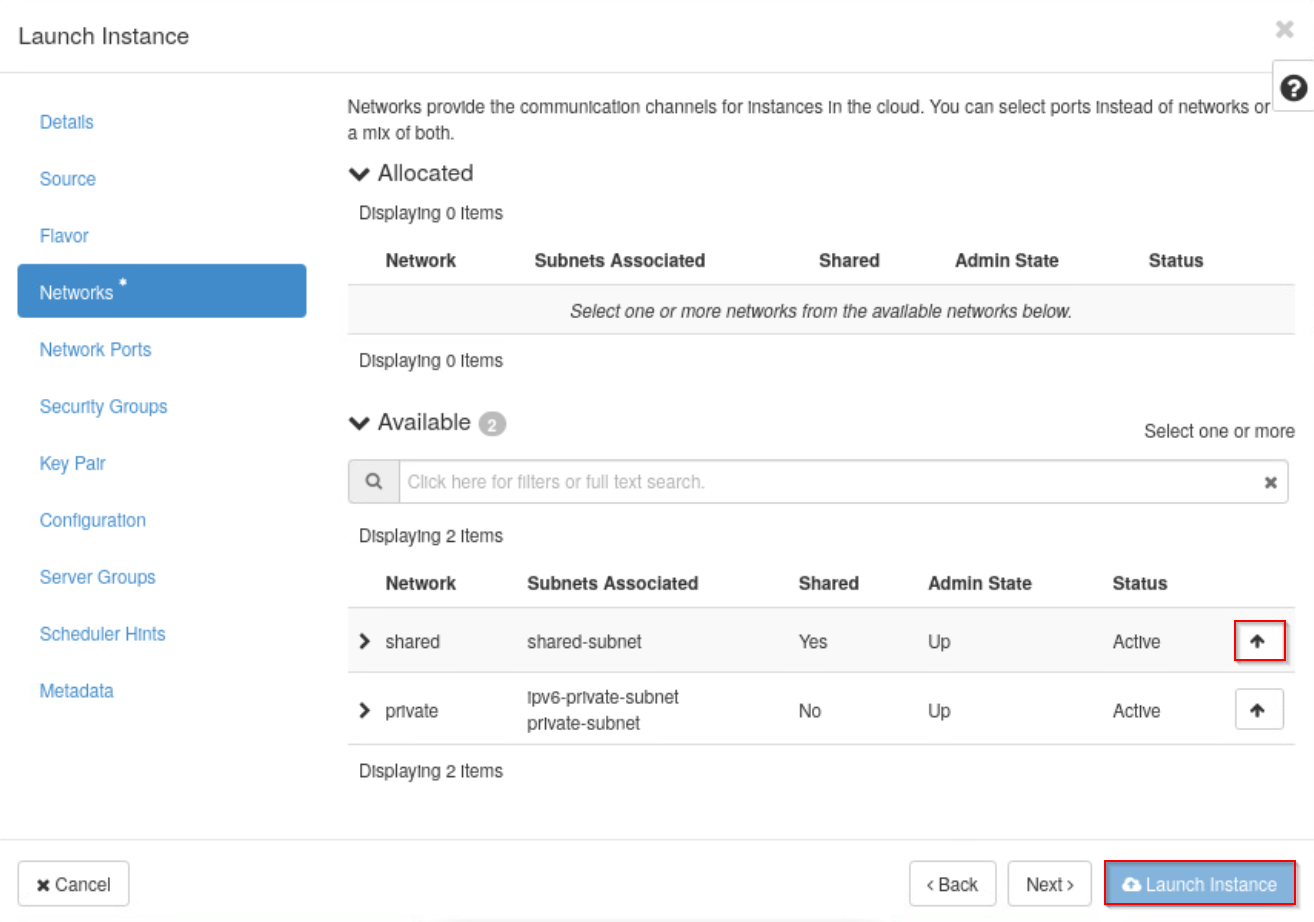
\includegraphics[width=\linewidth]{images/part1/step8.png}
        \end{center}
    \end{labstep}

    \begin{stopbox}
        Before proceeding to the next step, confirm that \textbf{shared} appears underneath the \textit{Allocated} section.
    \end{stopbox}

    \begin{labstep}
        Access the instance's console by clicking on \textbf{instance1} under the \textit{Instance Name} column.
        Then, navigate to the \textit{Console} tab if you are not directed there automatically.
        Click on \textbf{Click here to show only the console}.

        \begin{center}
            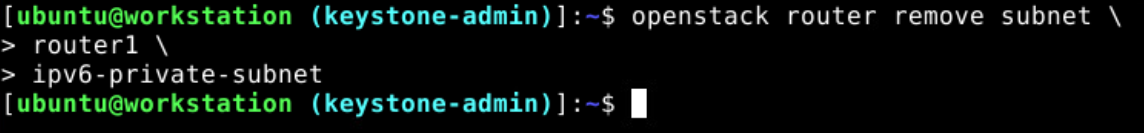
\includegraphics[width=\linewidth]{images/part1/step9.png}
        \end{center}
    \end{labstep}

    \begin{labstep}
        Log into the instance as \textbf{root} with the password \textbf{secret}.

        \begin{center}
            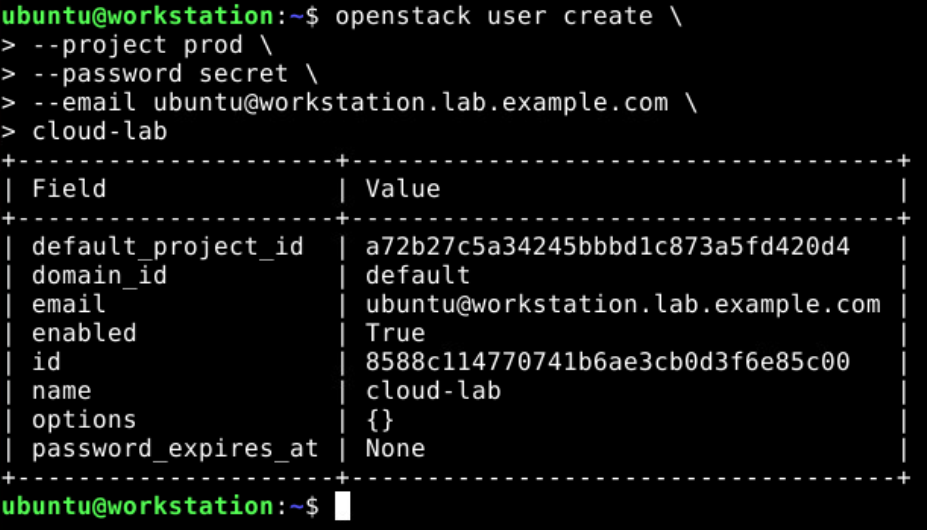
\includegraphics[width=\linewidth]{images/part1/step10.png}
        \end{center}
    \end{labstep}

    \begin{notebox}
        It may take several minutes for the instance to fully boot up and present a login prompt.
    \end{notebox}

    \begin{labstep}
        Now, we will make a change to the instance and create a snapshot.
        Create the \textbf{/root/hello.txt} file with the contents \textbf{Hello, world!}.
        \begin{lstlisting}
            root@instance1:~# echo 'Hello, world!' > /root/hello.txt
        \end{lstlisting}

        \begin{center}
            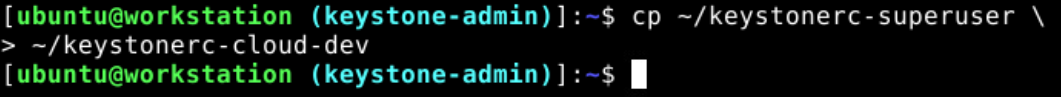
\includegraphics[width=\linewidth]{images/part1/step11.png}
        \end{center}
    \end{labstep}

    \begin{labstep}
        Now, navigate back to \textbf{Project $>$ Compute $>$ Instances}.
        Before creating a snapshot, click the dropdown next to \textbf{Create Snapshot} in the same row as \textbf{instance1}, then click \textbf{Shut Off Instance}.
        This will prevent any inconsistencies in the resulting snapshot.

        \begin{center}
            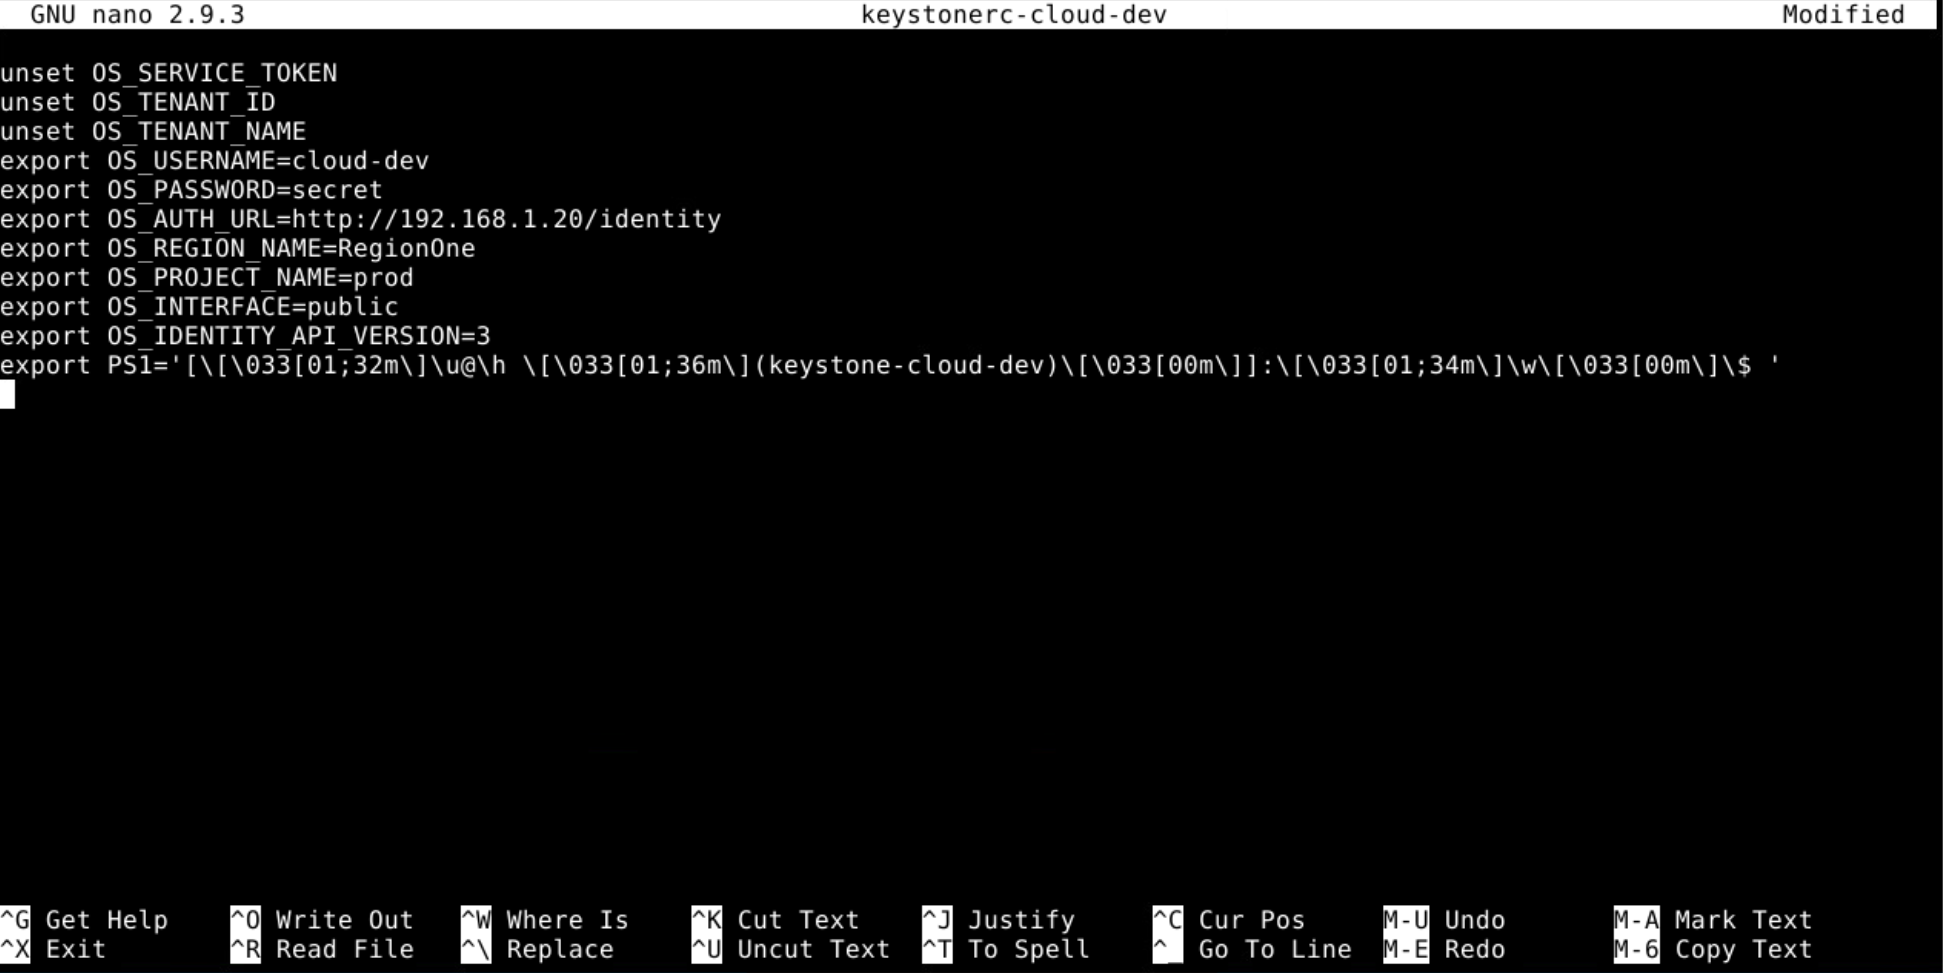
\includegraphics[width=\linewidth]{images/part1/step12.png}
        \end{center}
    \end{labstep}

    \begin{tipbox}
        A ``live snapshot'' is a snapshot of a running instance, which may only include a snapshot of the disk, while some OS state may be lost.
    \end{tipbox}
    \begin{notebox}
        Stopping instances and otherwise changing their running states will be explored further later in this lab.
    \end{notebox}

    \begin{labstep}
        When the \textit{Status} column shows that \textbf{instance1} is \textbf{Shutoff}, click \textbf{Create Snapshot}.

        \begin{center}
            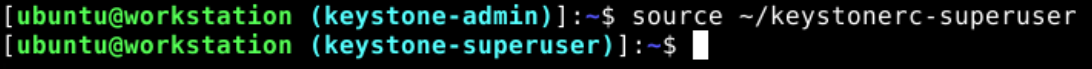
\includegraphics[width=\linewidth]{images/part1/step13.png}
        \end{center}
    \end{labstep}

    \begin{labstep}
        In the \textbf{Create Snapshot} dialog, enter \textbf{instance1-snapshot} in the \textit{Snapshot Name} field.
        Click \textbf{Create Snapshot}.

        \begin{center}
            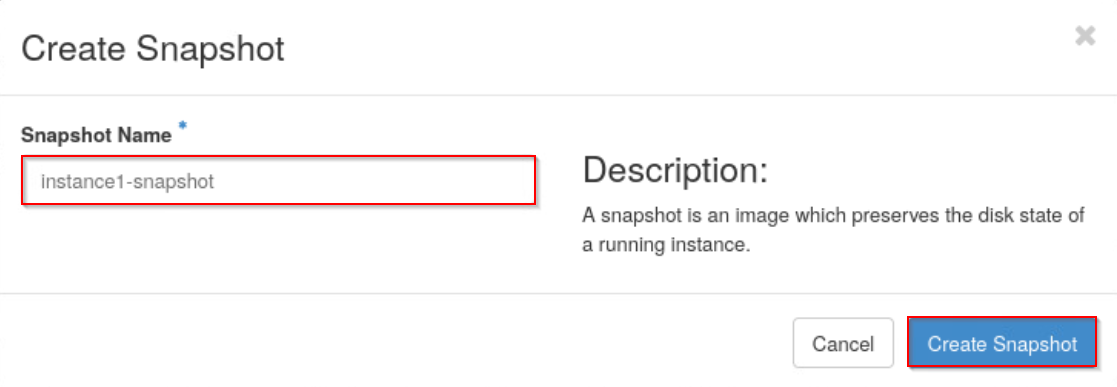
\includegraphics[width=\linewidth]{images/part1/step14.png}
        \end{center}
    \end{labstep}

    \begin{stopbox}
        When you create the snapshot, you will be redirected to \textbf{Projects $>$ Compute $>$ Images}.
        Wait until \textbf{instance1-snapshot} is \textbf{Active} before proceeding.
    \end{stopbox}

    \begin{labstep}
        Navigate back to the \textbf{Instances} page.
        The instance is no longer needed, so select the checkbox next to \textbf{instance1} and click \textbf{Delete Instances}.

        \begin{center}
            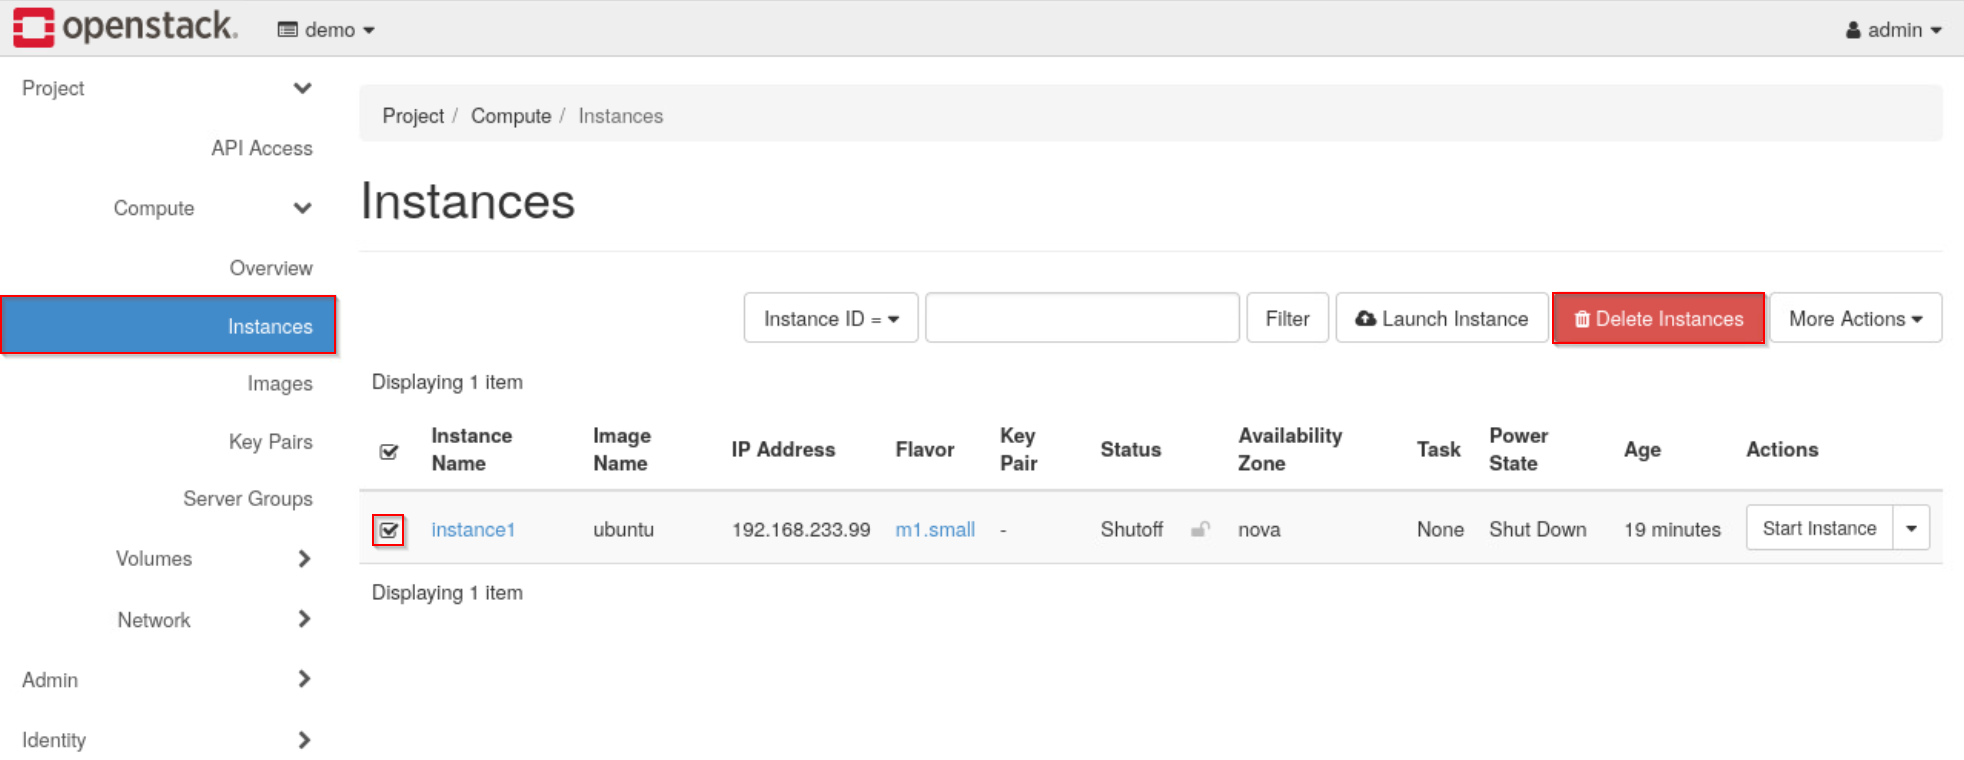
\includegraphics[width=\linewidth]{images/part1/step15.png}
        \end{center}
    \end{labstep}

    \begin{labstep}
        In the \textbf{Confirm Delete Instances} dialog, click \textbf{Delete Instances}.

        \begin{center}
            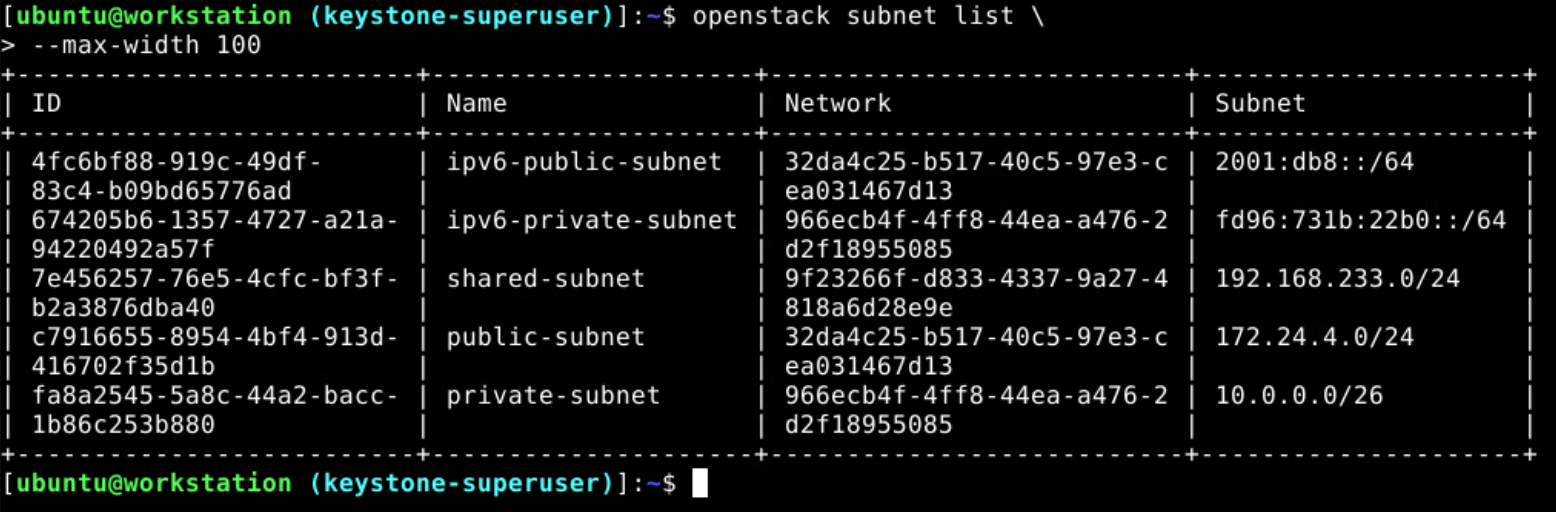
\includegraphics[width=\linewidth]{images/part1/step16.png}
        \end{center}
    \end{labstep}

    \begin{labstep}
        To verify that the snapshot works correctly, use the snapshot to launch another instance named \textbf{instance1}.
        Follow the same steps that were used to create \textbf{instance1}.
        However, in the \textit{Source} tab of the \textbf{Launch Instance} dialog, select \textbf{Image Snapshot} under \textit{Boot Source} click the $\uparrow$ symbol next to \textbf{instance1-snapshot}.

        \begin{center}
            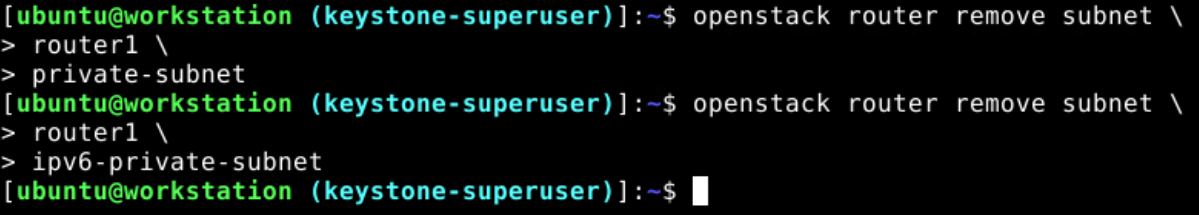
\includegraphics[width=\linewidth]{images/part1/step17.png}
        \end{center}
    \end{labstep}

    \begin{tipbox}
        The snapshot will also appear on the \textbf{Project $>$ Compute $>$ Images} page.
        It should say \textbf{Snapshot} in the \textit{Type} column.
        For an alternative method of launching an image with the snapshot, navigate to this page, click \textbf{Launch} in the same row as the snapshot, and enter the required information in the following dialog.
        The snapshot can also be deleted from here.
    \end{tipbox}

    \begin{labstep}
        Open the instance's console and log in with the username \textbf{root} and password \textbf{secret}.
        Check that the file created in the previous instance also exists on this instance.
        \begin{lstlisting}
            root@instance1:~# cat /root/hello.txt
        \end{lstlisting}

        \begin{center}
            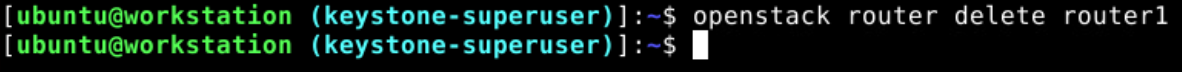
\includegraphics[width=\linewidth]{images/part1/step18.png}
        \end{center}
    \end{labstep}

    \begin{notebox}
        It may take several minutes for the instance to fully boot up and present a login prompt.
    \end{notebox}

    \begin{labstep}
        Exit the instance's console, navigate back to \textbf{Project $>$ Compute $>$ Instances}, and delete the instance.

        \begin{center}
            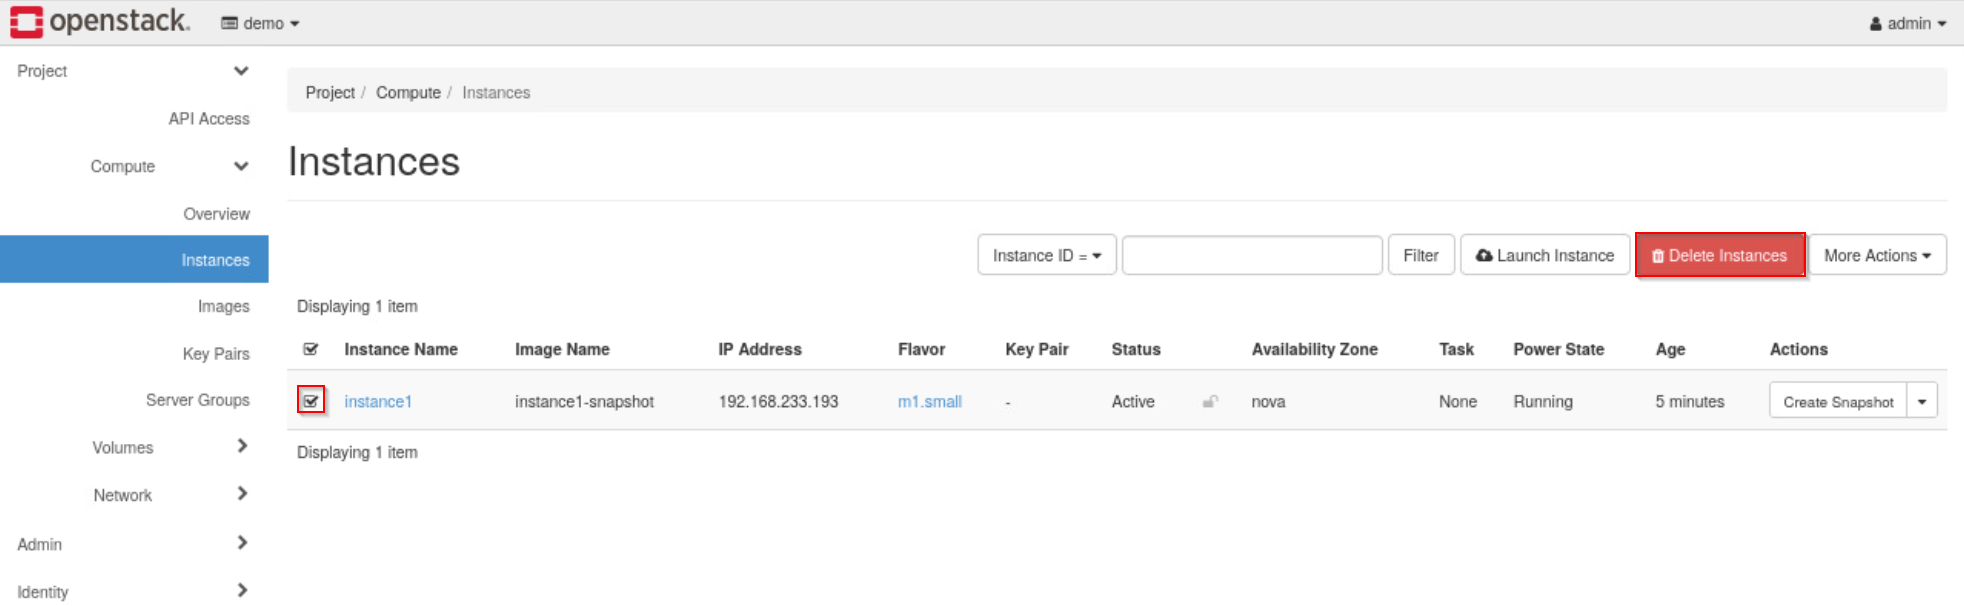
\includegraphics[width=\linewidth]{images/part1/step19.png}
        \end{center}
    \end{labstep}

    \begin{labstep}
        You will create another snapshot with the \textit{OpenStack Unified CLI} in the next task, so \textbf{instance1-snapshot} can safely be deleted.
        Navigate to \textbf{Project $>$ Compute $>$ Images}, select \textbf{instance1-snapshot}, and click \textbf{Delete Images}.

        \begin{center}
            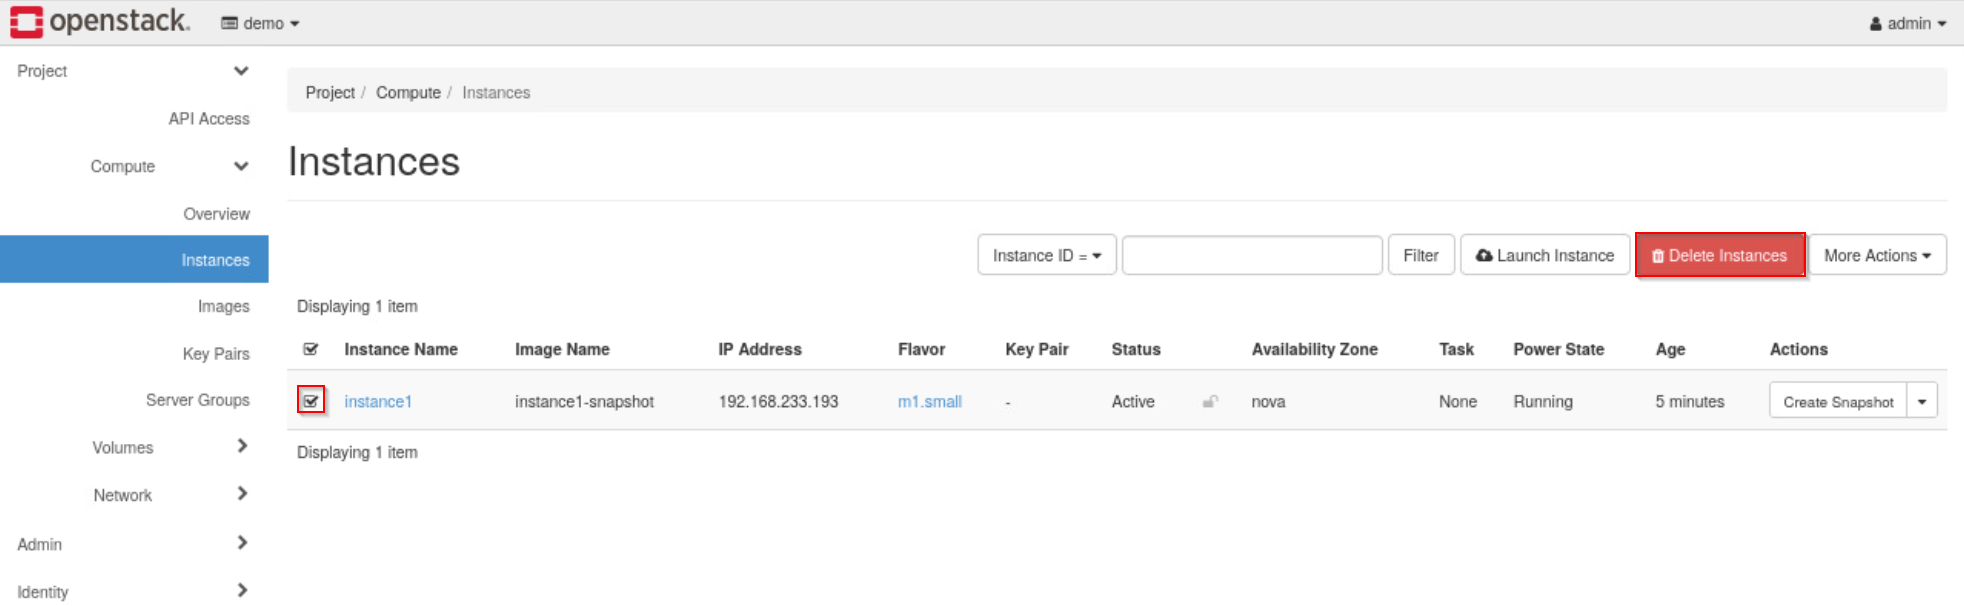
\includegraphics[width=\linewidth]{images/part1/step20.png}
        \end{center}
    \end{labstep}

    \begin{labstep}
        In the \textbf{Confirm Delete Image} dialog, click \textbf{Delete Image}.

        \begin{center}
            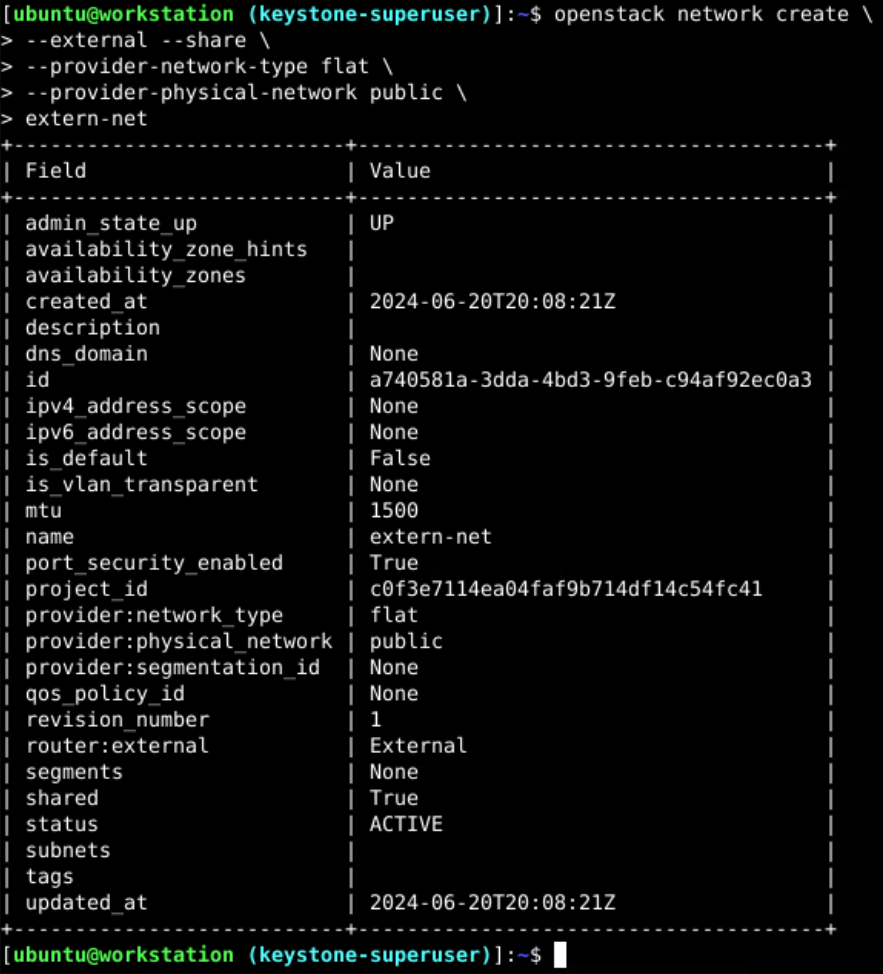
\includegraphics[width=\linewidth]{images/part1/step21.png}
        \end{center}
    \end{labstep}

    \begin{labstep}
        Log out of the dashboard, close the browser window, and continue to the next task.
    \end{labstep}
\end{enumerate}

%%%%%%%%%%%
% Section 2
%%%%%%%%%%%
\section{Creating a Snapshot with the OpenStack Unified CLI}\label{sec:creating_a_snapshot_cli}
In this task, you will repeat the steps from the previous task in the \textit{OpenStack Unified CLI}.

\begin{enumerate}
    \begin{labstep}
        Open a terminal window and source the keystone credentials for the \textbf{admin} user.
        \begin{lstlisting}
            ubuntu@workstation:~$ source ~/keystonerc-admin
        \end{lstlisting}

        \begin{center}
            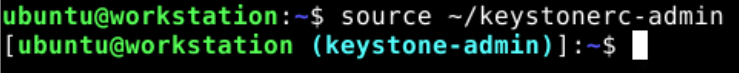
\includegraphics[width=\linewidth]{images/part2/step1.png}
        \end{center}
    \end{labstep}

    \begin{labstep}
        List the current instances.
        The list should be empty.
        \begin{lstlisting}
            [ubuntu@workstation (keystone-admin)]:~$ openstack server list
        \end{lstlisting}

        \begin{center}
            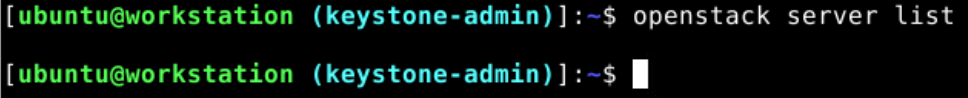
\includegraphics[width=\linewidth]{images/part2/step2.png}
        \end{center}
    \end{labstep}

    \begin{labstep}
        Now, we will create the same snapshot as before from the command line.
        Launch an instance.
        Use the \textbf{ubuntu} image, the \textbf{m1.small} flavor, and the \textbf{shared} network.
        \begin{lstlisting}
            [ubuntu@workstation (keystone-admin)]:~$ openstack server create \
            > --image ubuntu \
            > --flavor m1.small \
            > --nic net-id=shared \
            instance2
        \end{lstlisting}

        \begin{center}
            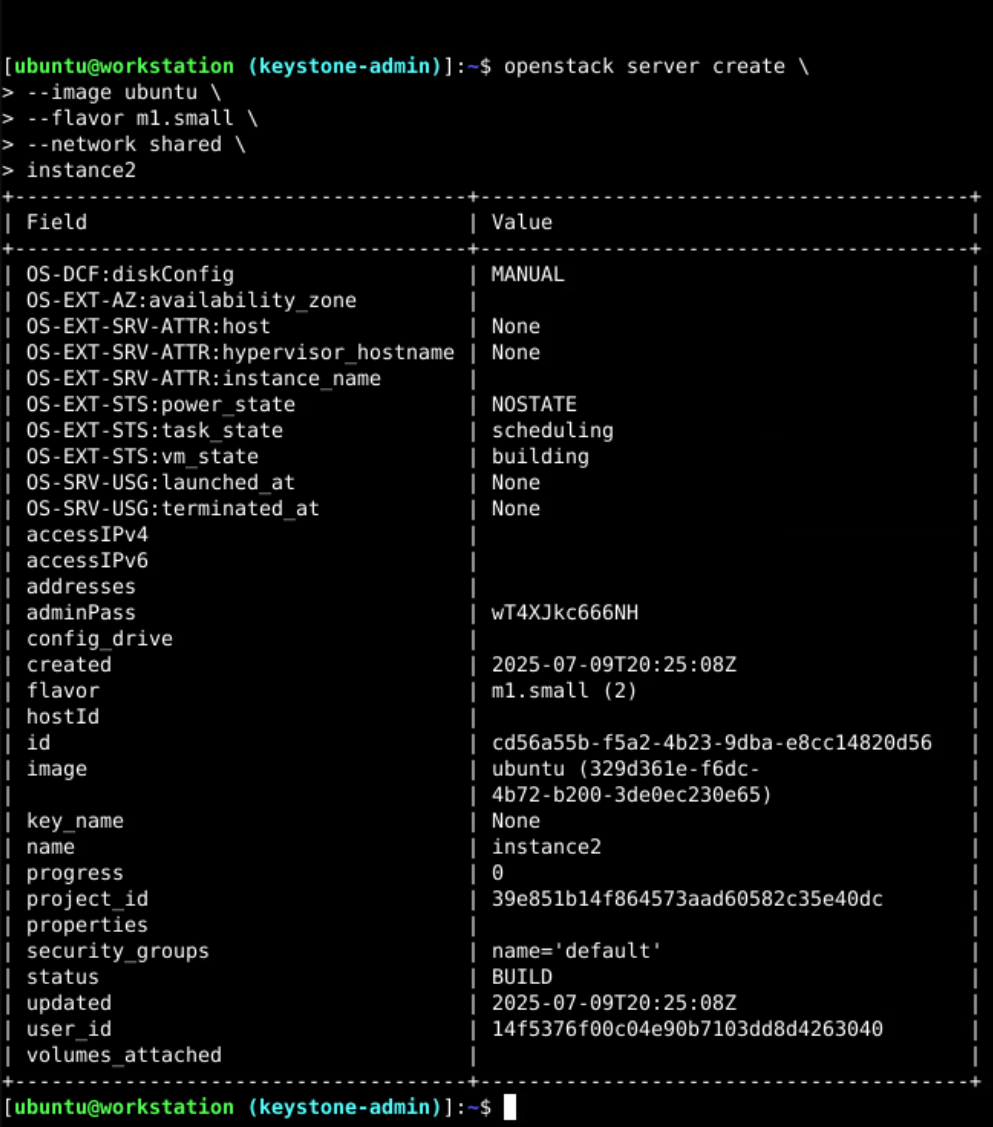
\includegraphics[width=\linewidth]{images/part2/step3.png}
        \end{center}
    \end{labstep}

    \begin{labstep}
        List the instances again to ensure it was created correctly.
        \begin{lstlisting}
            [ubuntu@workstation (keystone-admin)]:~$ openstack server list \
            > --max-width 80
        \end{lstlisting}

        \begin{center}
            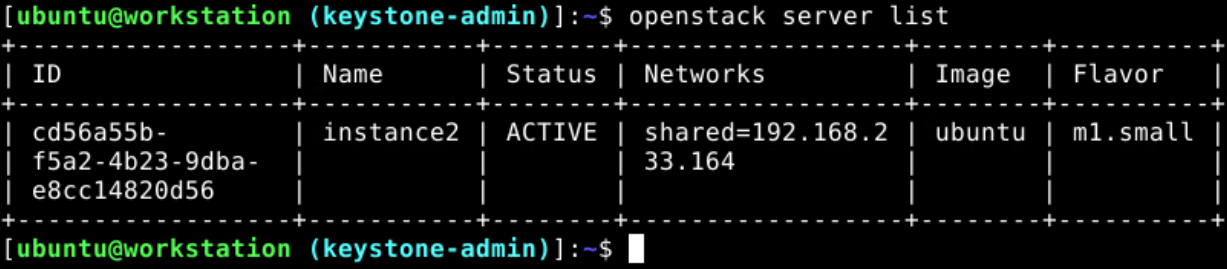
\includegraphics[width=\linewidth]{images/part2/step4.png}
        \end{center}
    \end{labstep}

    \begin{tipbox}
        When typing the command, make sure there is a space between \textbf{list} and the \textbf{\textbackslash} character, and press \textbf{Enter} to get the \textbf{$>$} and continue typing the rest of the command.
    \end{tipbox}

    \begin{labstep}
        Show the URL to the console of the instance.
        Right-click the URL and click \textbf{Open Link}.
        \begin{lstlisting}
            [ubuntu@workstation (keystone-admin)]:~$ openstack console url show instance2
        \end{lstlisting}

        \begin{center}
            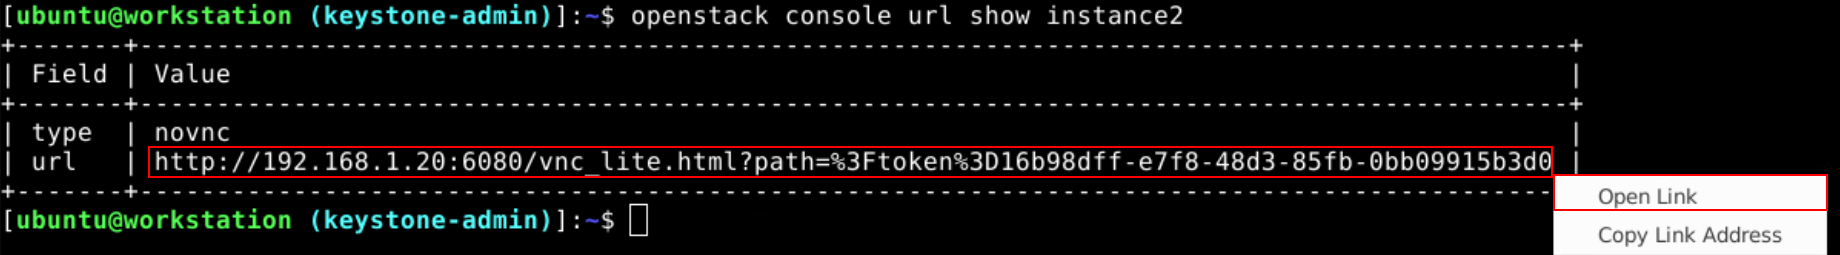
\includegraphics[width=\linewidth]{images/part2/step5.png}
        \end{center}
    \end{labstep}

    \begin{labstep}
        Log in to \textbf{instance2} as \textbf{root} with the password \textbf{secret}.

        \begin{center}
            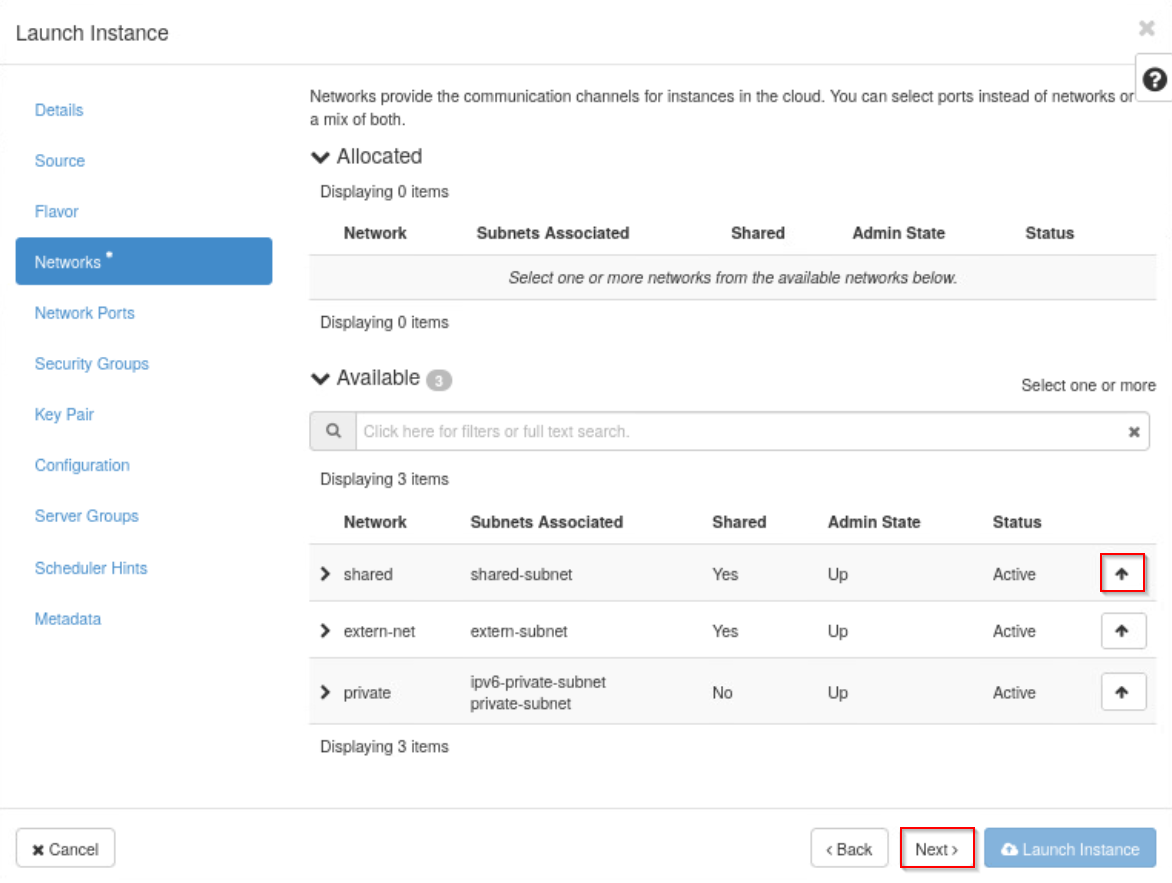
\includegraphics[width=\linewidth]{images/part2/step6.png}
        \end{center}
    \end{labstep}

    \begin{notebox}
        It may take several minutes for the instance to fully boot up and present a login prompt.
    \end{notebox}

    \begin{labstep}
        Create the \textbf{/root/hello.txt} file with the contents \textbf{Hello, world!}.
        \begin{lstlisting}
            root@instance2:~# echo 'Hello, world!' > /root/hello.txt
        \end{lstlisting}

        \begin{center}
            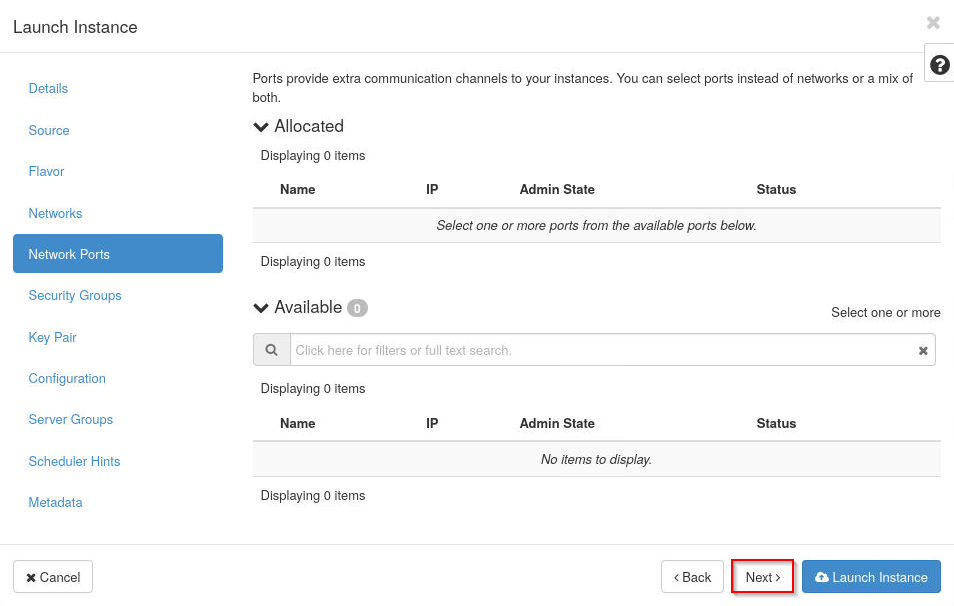
\includegraphics[width=\linewidth]{images/part2/step7.png}
        \end{center}
    \end{labstep}

    \begin{labstep}
        Close the browser window and return focus to the terminal window.
        Stop the instance before making a snapshot.
        \begin{lstlisting}
            [ubuntu@workstation (keystone-admin)]:~$ openstack server stop instance2
        \end{lstlisting}

        \begin{center}
            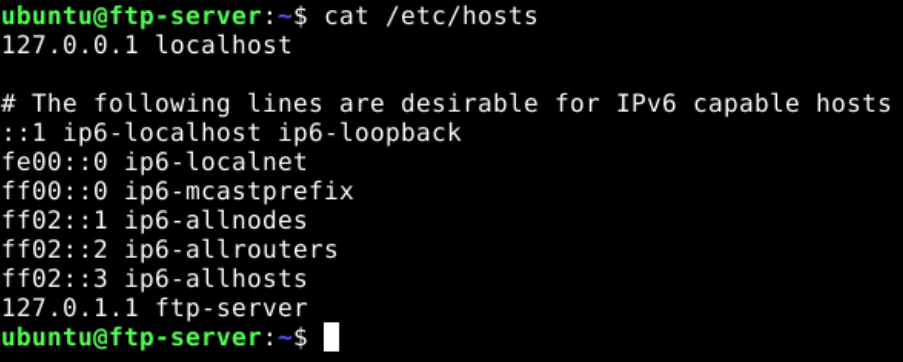
\includegraphics[width=\linewidth]{images/part2/step8.png}
        \end{center}
    \end{labstep}

    \begin{labstep}
        List the current images.
        The list should have two items.
        \begin{lstlisting}
            [ubuntu@workstation (keystone-admin)]:~$ openstack image list
        \end{lstlisting}

        \begin{center}
            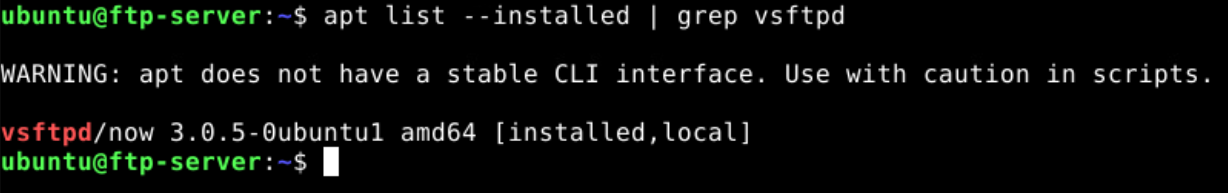
\includegraphics[width=\linewidth]{images/part2/step9.png}
        \end{center}
    \end{labstep}

    \begin{labstep}
        Make a snapshot of the instance.
        \begin{lstlisting}
            [ubuntu@workstation (keystone-admin)]:~$ openstack server image create \
            > instance2 \
            > --name instance2-snapshot \
            > --max-width 80
        \end{lstlisting}

        \begin{center}
            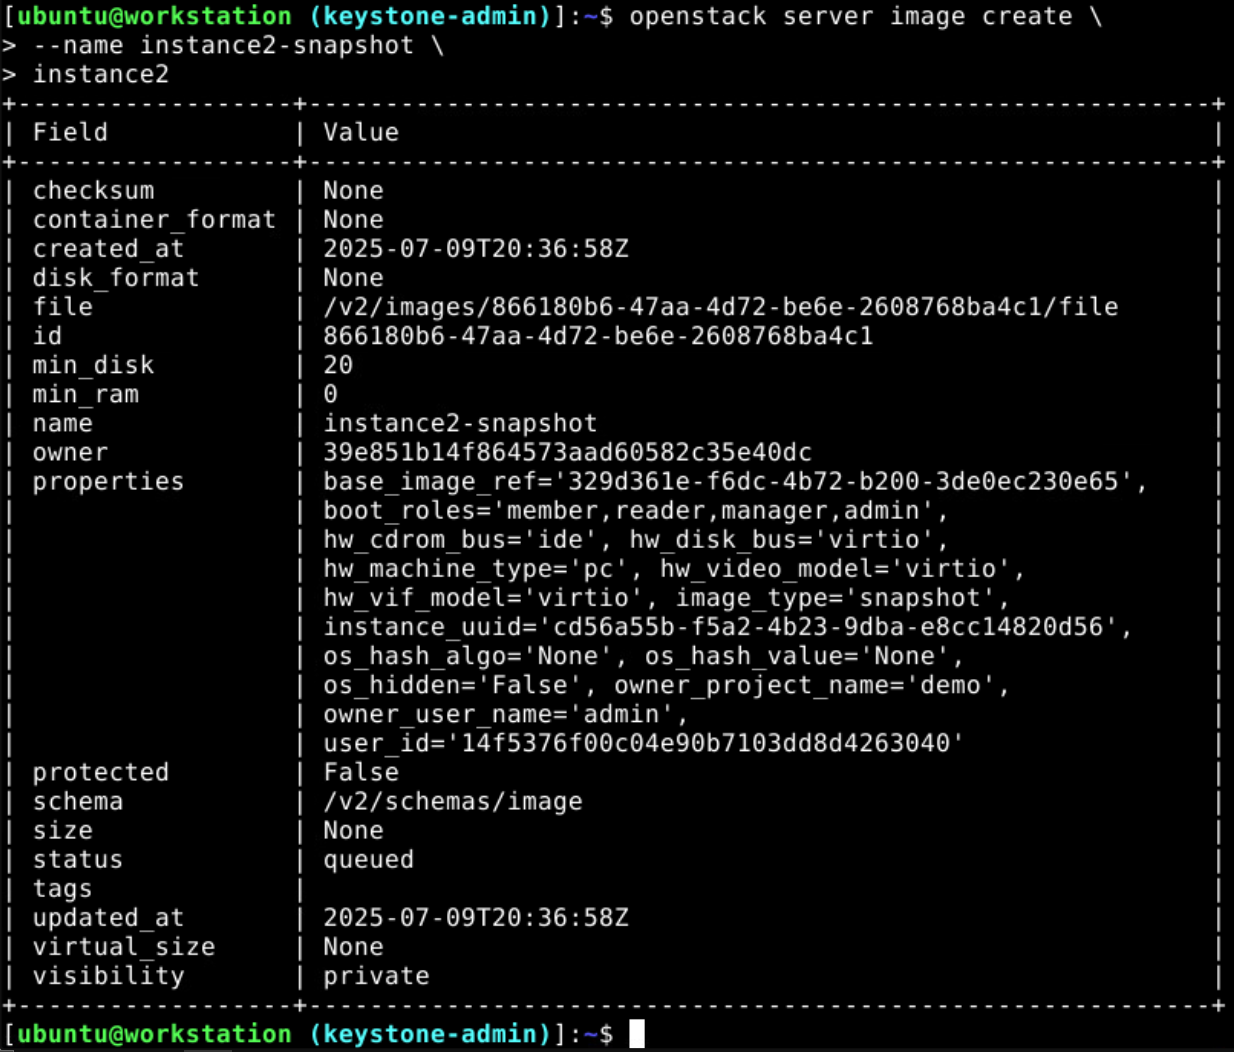
\includegraphics[width=\linewidth]{images/part2/step10.png}
        \end{center}
    \end{labstep}

    \begin{labstep}
        List the current images again to ensure the snapshot was created properly.
        \begin{lstlisting}
            [ubuntu@workstation (keystone-admin)]:~$ openstack image list
        \end{lstlisting}

        \begin{center}
            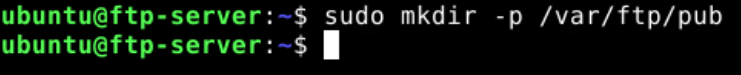
\includegraphics[width=\linewidth]{images/part2/step11.png}
        \end{center}
    \end{labstep}

    \begin{labstep}
        To verify the correctness of the snapshot, first delete the instance.
        \begin{lstlisting}
            [ubuntu@workstation (keystone-admin)]:~$ openstack server delete instance2
        \end{lstlisting}

        \begin{center}
            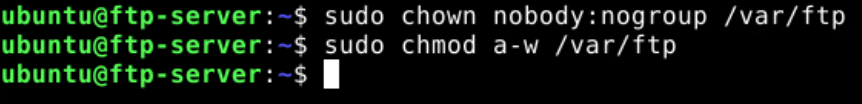
\includegraphics[width=\linewidth]{images/part2/step12.png}
        \end{center}
    \end{labstep}

    \begin{labstep}
        Confirm the deletion of the instance.
        \begin{lstlisting}
            [ubuntu@workstation (keystone-admin)]:~$ openstack server list
        \end{lstlisting}

        \begin{center}
            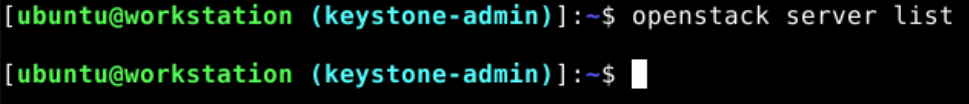
\includegraphics[width=\linewidth]{images/part2/step13.png}
        \end{center}
    \end{labstep}

    \begin{labstep}
        Now, recreate the instance, using \textbf{instance2-snapshot} as the image.
        \begin{lstlisting}
            [ubuntu@workstation (keystone-admin)]:~$ openstack server create \
            > --image instance2-snapshot \
            > --flavor m1.small \
            > --nic net-id=shared \
            instance2
        \end{lstlisting}

        \begin{center}
            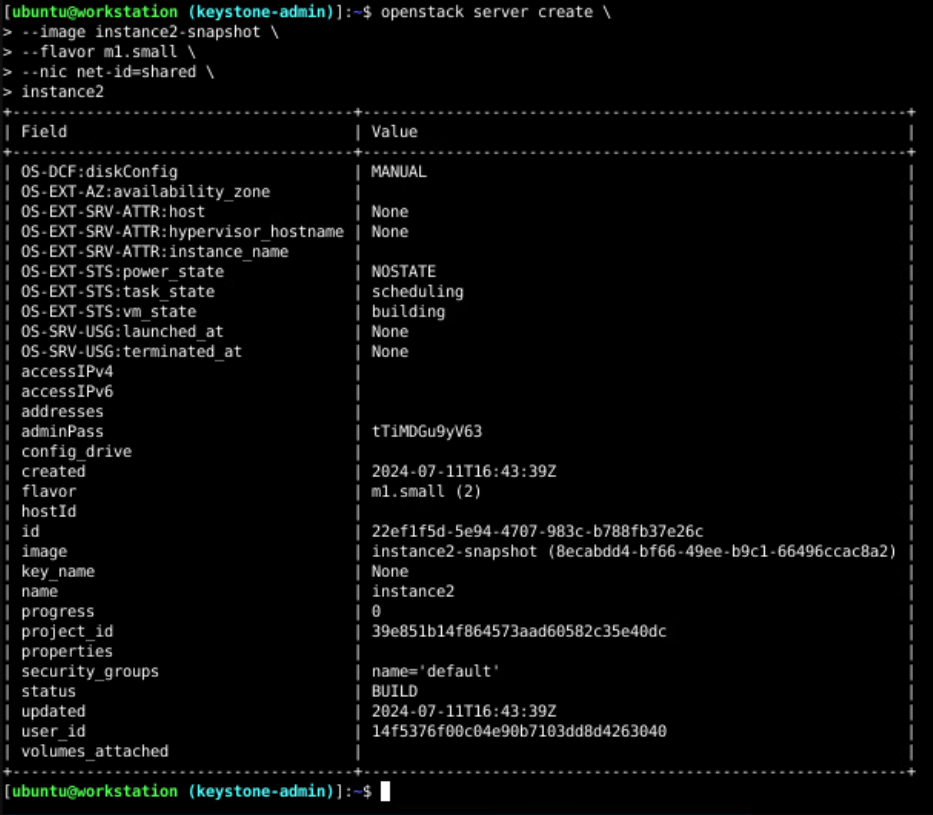
\includegraphics[width=\linewidth]{images/part2/step14.png}
        \end{center}
    \end{labstep}

    \begin{labstep}
        Using the same steps as before, log in to the instance's console as \textbf{root} with the password \textbf{secret}.
        Verify that the \textbf{/root/hello.txt} file exists.
        \begin{lstlisting}
            root@instance2:~# cat /root/hello.txt
        \end{lstlisting}

        \begin{center}
            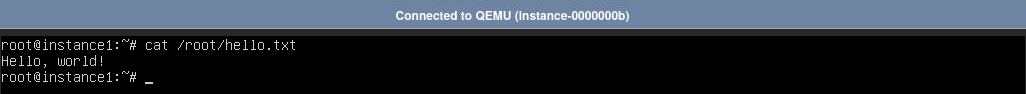
\includegraphics[width=\linewidth]{images/part2/step15.png}
        \end{center}
    \end{labstep}

    \begin{notebox}
        It may take several minutes for the instance to fully boot up and present a login prompt.
    \end{notebox}

    \begin{labstep}
        This instance will be used in the following sections.
        Leave both the browser and terminal windows open and continue to the next task.
    \end{labstep}

\end{enumerate}

% TODO: In the case that storage volumes are added to these labs, rescuing instances should be discussed in the following two
% sections.

%%%%%%%%%%%
% Section 3
%%%%%%%%%%%
\section{Managing the Running State of an Instance with the Horizon Dashboard}\label{sec:managing_the_running_state_of_an_instance_web}
OpenStack allows for managing the running and power state of instances in a variety of ways, and each method may be useful in different situations.
In this task, you will manage the running and power state of an instance by starting, stopping, pausing, suspending, resuming, shelving, unshelving, and rebooting the instance with the \textit{Horizon Dashboard}.

\begin{enumerate}
    \begin{labstep}
        Open a new tab in the browser window and navigate to \textbf{192.168.1.20}.
        Log in as \textbf{admin} with the password \textbf{secret}.
    \end{labstep}

    \begin{labstep}
        Pausing an instance is one way to manage the running state of an OpenStack instance.
        When an instance is paused, its operation is frozen, and its state and memory are preserved in the RAM of the underlying compute node.
        Pausing an instance does not release its resources.
        When the instance is resumed, it will pick up any processes where they left off.
        To view the effects of pausing an instance, first focus back on the tab with the instance's console and continuously ping the DHCP server.
        \begin{lstlisting}
            root@instance2:~# ping 192.168.233.2
        \end{lstlisting}

        \begin{center}
            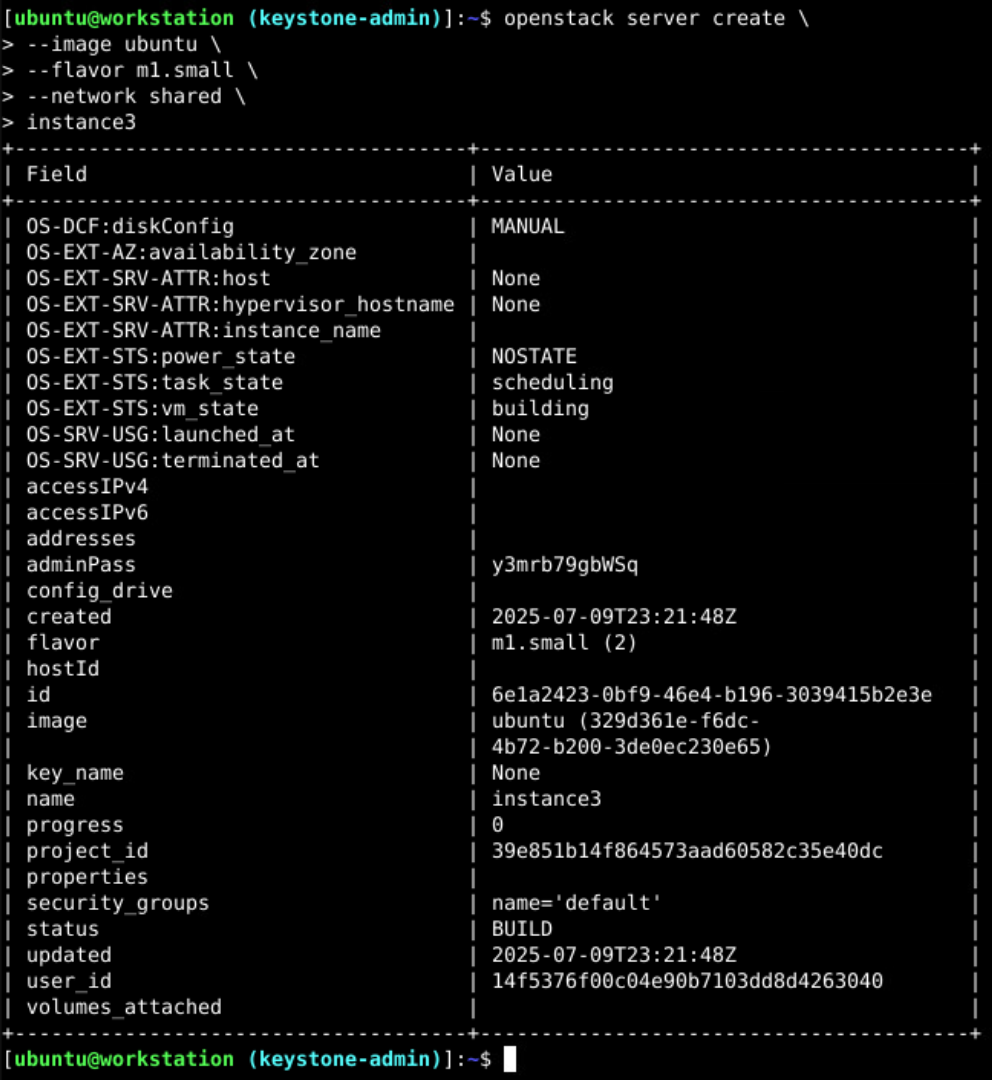
\includegraphics[width=\linewidth]{images/part3/step2.png}
        \end{center}
    \end{labstep}

    \begin{tipbox}
        Pausing an instance is useful when the operation of an instance needs to be interrupted while its state should be kept intact.
        For example, an instance might be paused while making changes to the underlying infrastructure to prevent disrupting processes and requiring applications or the instance to be restarted.
        Pausing an instance is similar to putting a computer in sleep mode.
    \end{tipbox}

    \begin{labstep}
        To pause the instance, navigate to \textbf{Project $>$ Compute $>$ Instances}, click the dropdown next to \textbf{Create Snapshot} in the same row as \textbf{instance2}, and click \textbf{Pause Instance}.

        \begin{center}
            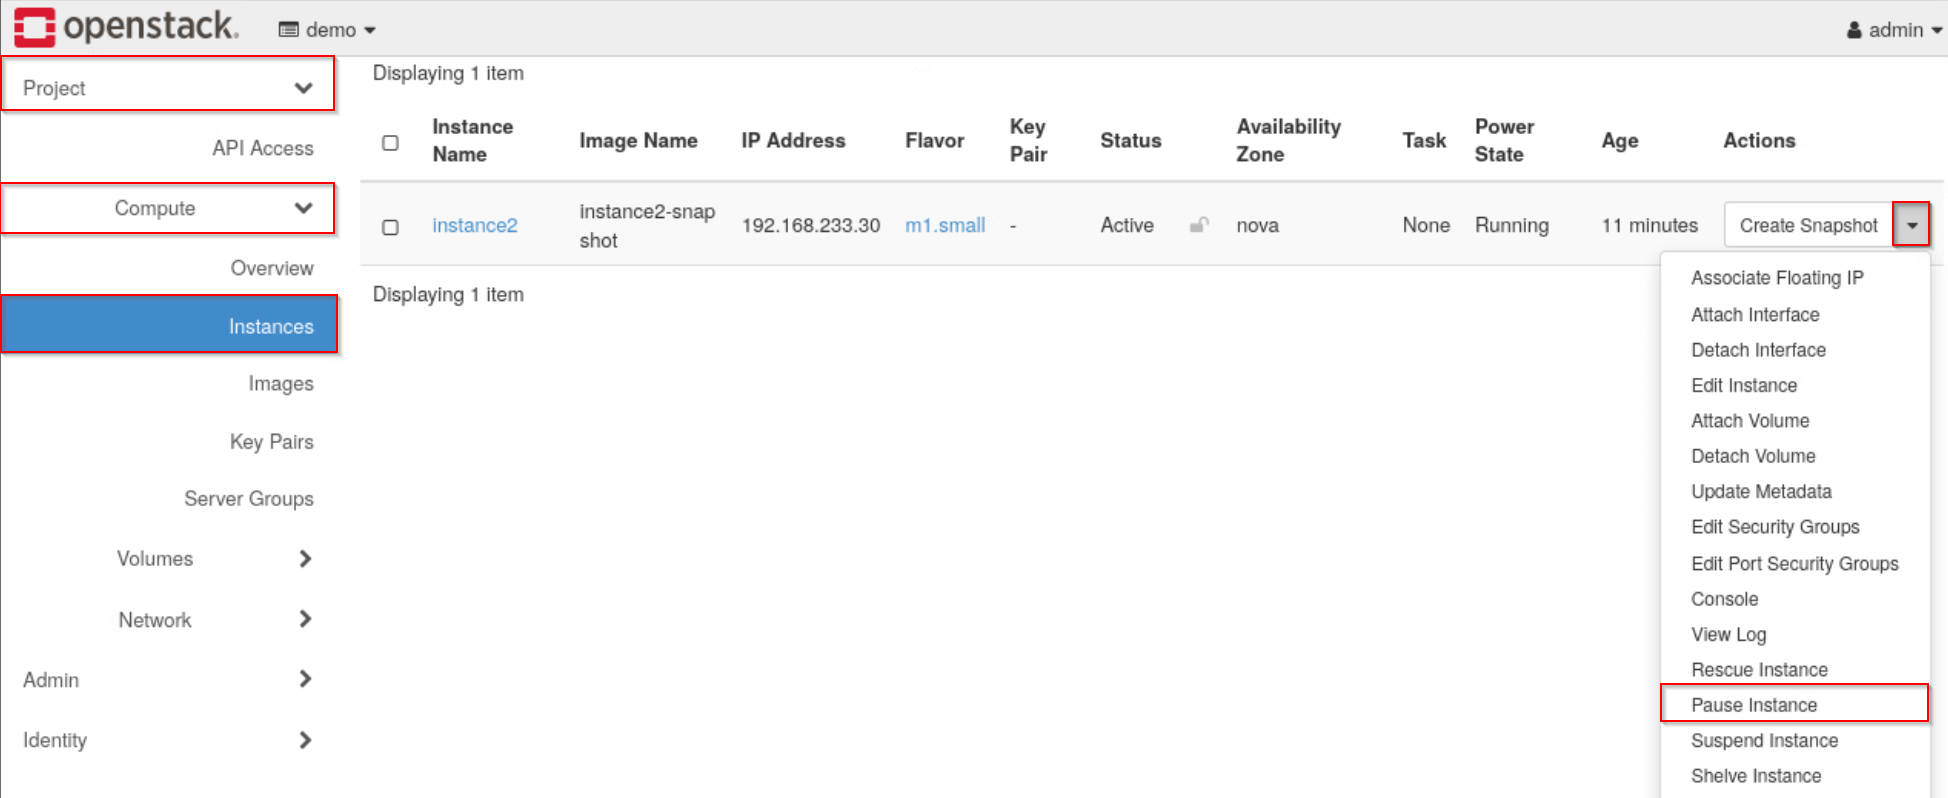
\includegraphics[width=\linewidth]{images/part3/step3.png}
        \end{center}
    \end{labstep}

    \begin{notebox}
        You may have to scroll down to find the option.
    \end{notebox}

    \begin{labstep}
        Now, view the console again to see that it is frozen and no more ping replies are appearing.

        \begin{center}
            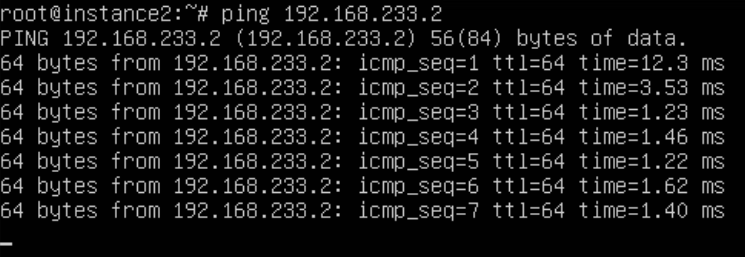
\includegraphics[width=\linewidth]{images/part3/step4.png}
        \end{center}
    \end{labstep}

    \begin{labstep}
        Navigate back to the \textbf{Instances} page.
        Click the dropdown next to \textbf{Create Snapshot} in the same row as \textbf{instance2} and click \textbf{Resume Instance}.

        \begin{center}
            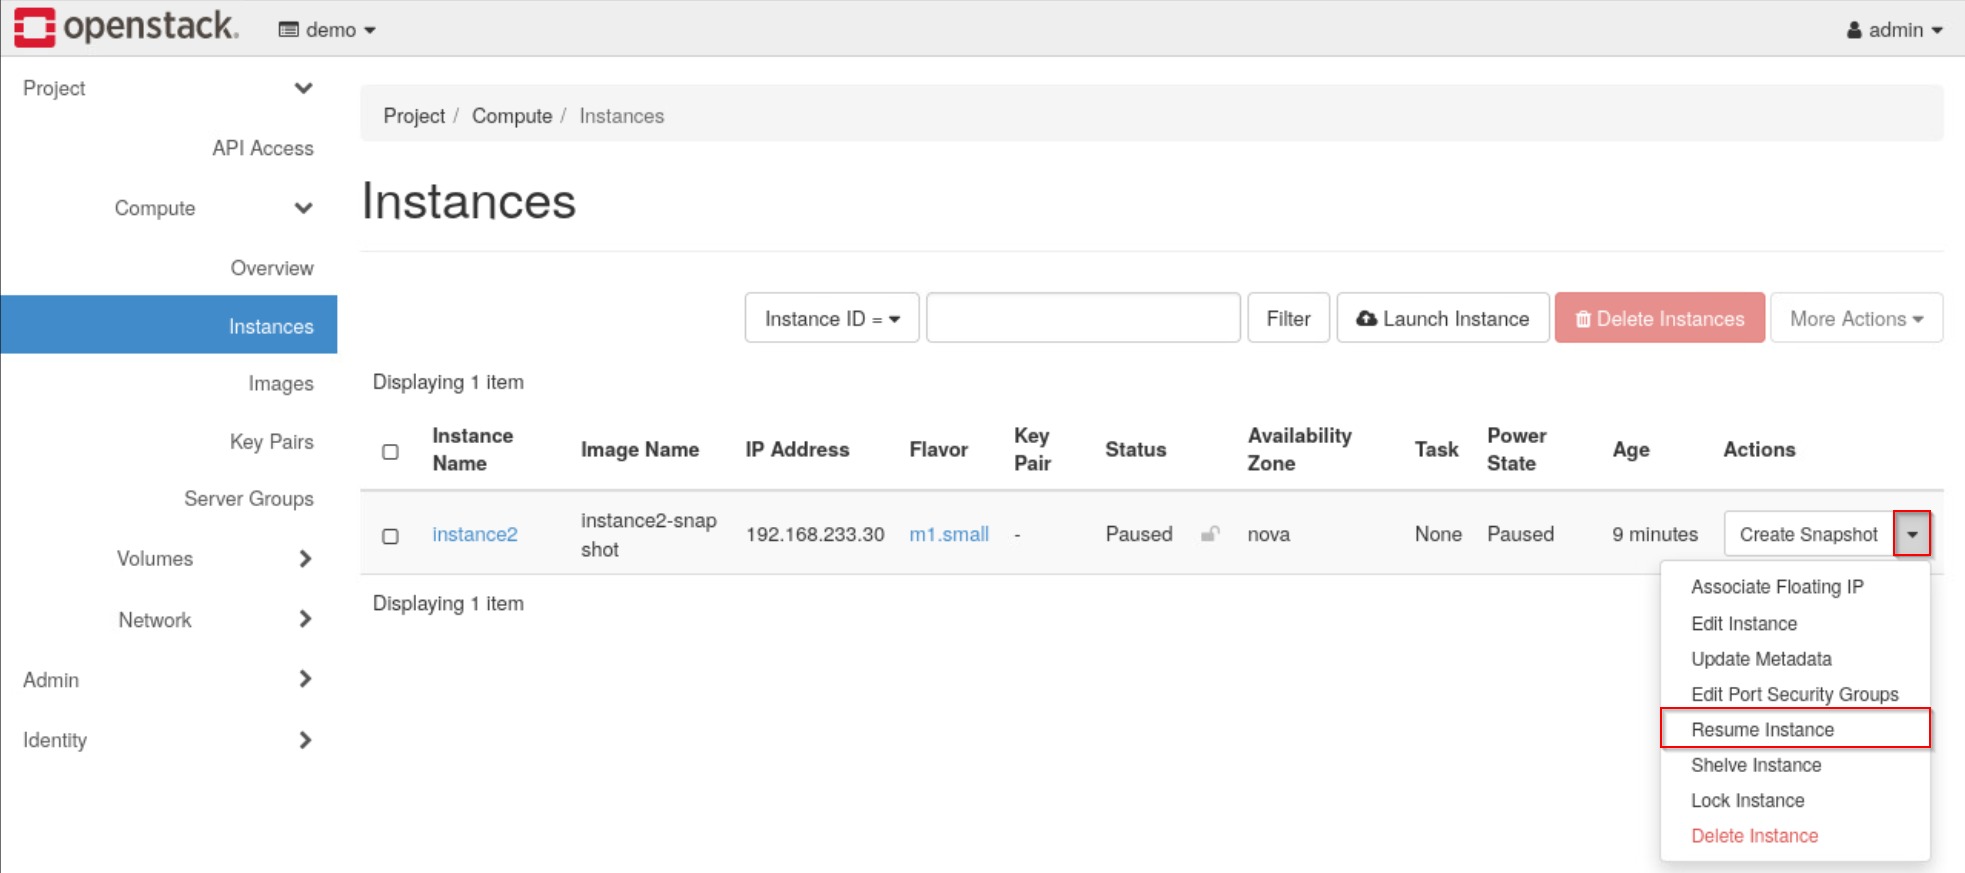
\includegraphics[width=\linewidth]{images/part3/step5.png}
        \end{center}
    \end{labstep}

    \begin{labstep}
        View the console again to see that the ping replies have resumed.
        Press \textbf{Ctrl+C} to stop the \textbf{ping} command.

        \begin{center}
            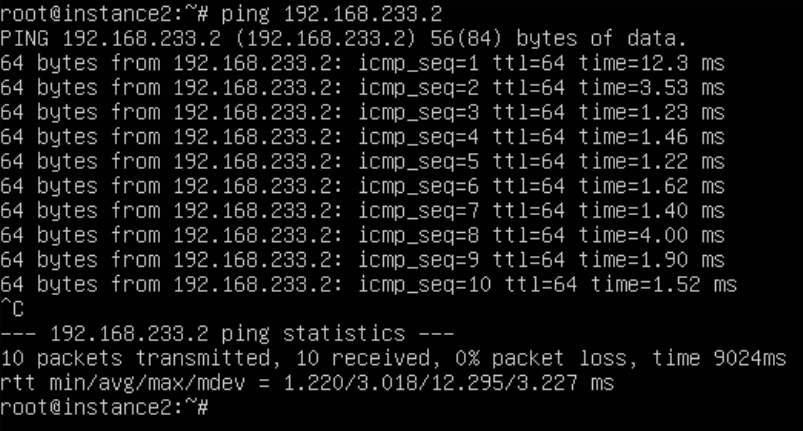
\includegraphics[width=\linewidth]{images/part3/step6.png}
        \end{center}
    \end{labstep}

    \begin{labstep}
        Suspending an instance is similar to pausing an instance.
        The main difference is that the instance's state is written to a persistent disk of the underlying compute node rather than memory.
        This means the state can be preserved even if the compute node loses power during the suspension.
        Suspending an instance does not release its resources.
        When the instance is resumed, it will pick up any processes where they left off.
        To view the effects of suspending an instance, perform the same experiment as before.
        Focus on the tab with the instance's console and continuously ping the DHCP server.
        \begin{lstlisting}
            root@instance2:~# ping 192.168.233.2
        \end{lstlisting}

        \begin{center}
            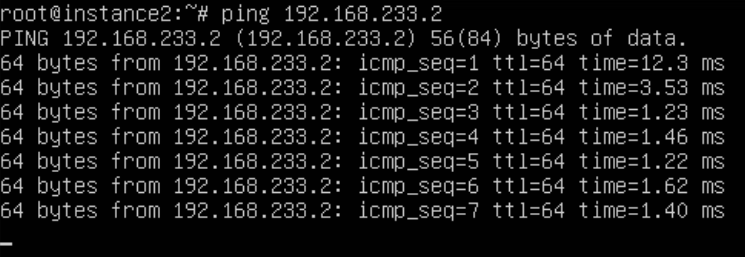
\includegraphics[width=\linewidth]{images/part3/step7.png}
        \end{center}
    \end{labstep}

    \begin{tipbox}
        Suspending an instance is useful in similar situations as pausing.
        However, suspending an image allows the compute node to be rebooted or migrated without disrupting the processes of the instance and requiring applications or the instance to be restarted.
        Suspending an instance is similar to putting a computer in hibernation mode.
    \end{tipbox}

    \begin{labstep}
        To suspend the instance, navigate back to \textbf{Project $>$ Compute $>$ Instances}, click the dropdown next to \textbf{Create Snapshot}, and click \textbf{Suspend Instance}.

        \begin{center}
            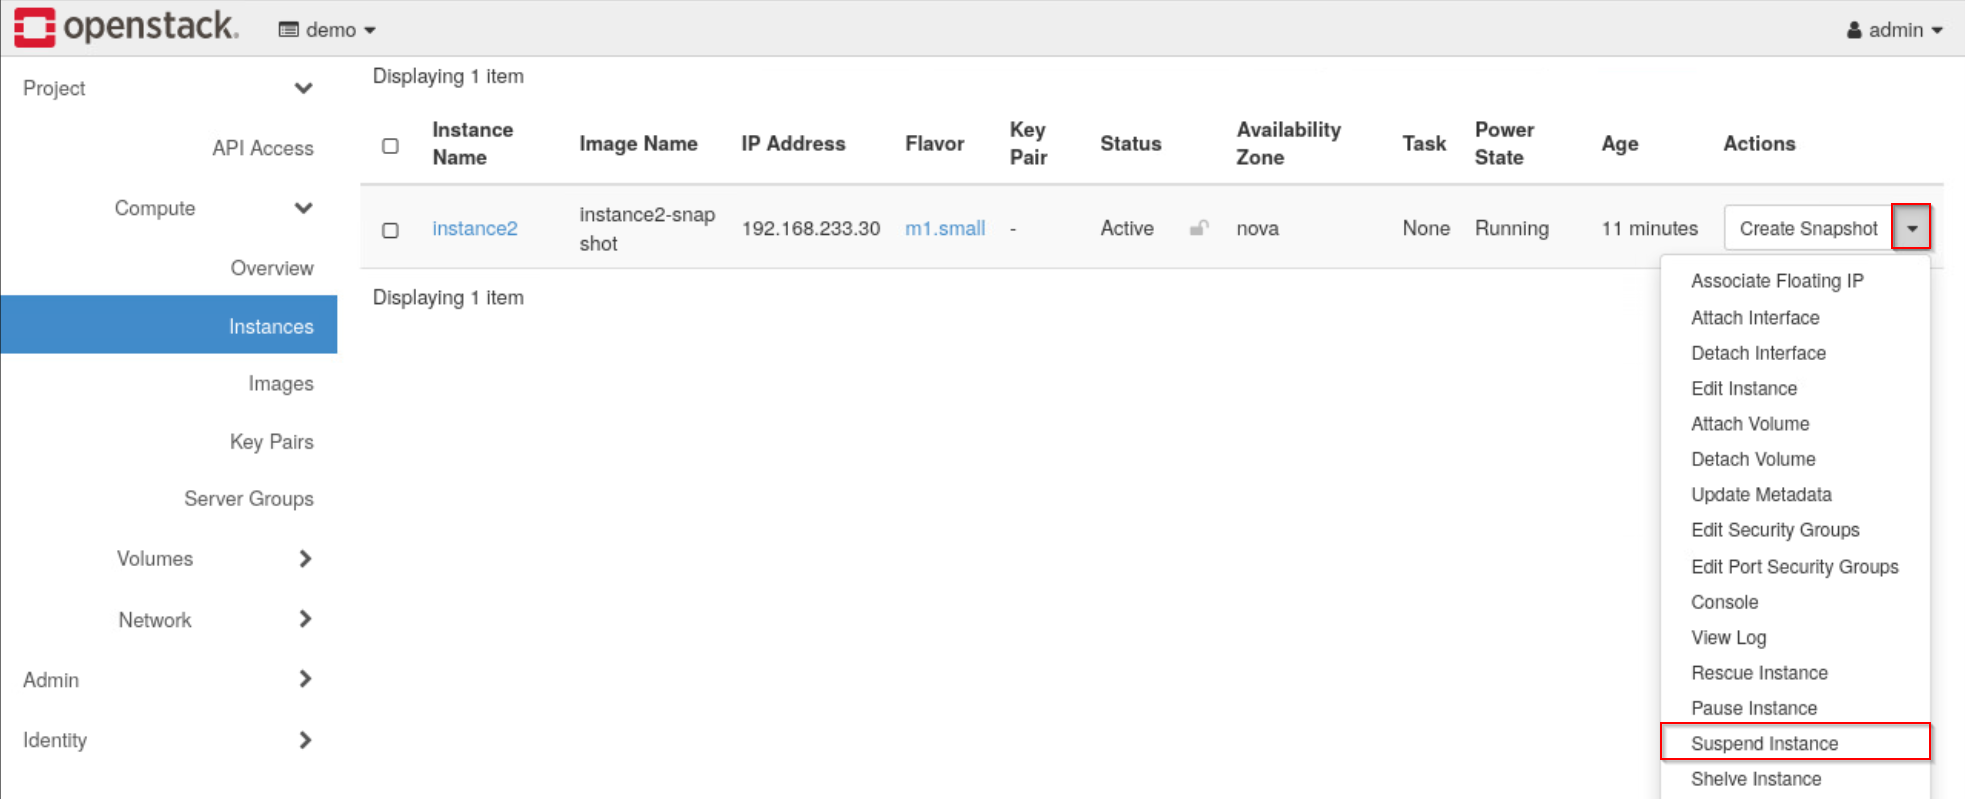
\includegraphics[width=\linewidth]{images/part3/step8.png}
        \end{center}
    \end{labstep}

    \begin{notebox}
        You may have to scroll down to find the option.
    \end{notebox}

    \begin{labstep}
        View the console again to see that the connection has been ended.
        When the instance is resumed, a new connection will be created, and this tab will still be unresponsive.
        Close the tab containing the instance console.

        \begin{center}
            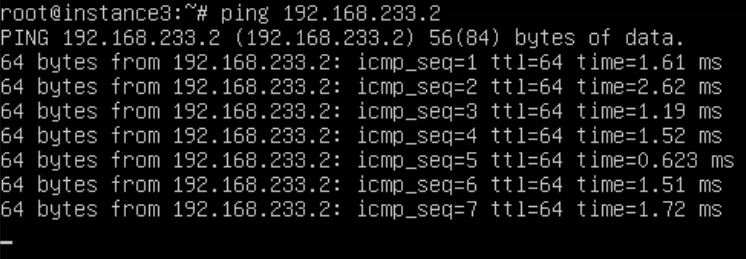
\includegraphics[width=\linewidth]{images/part3/step9.png}
        \end{center}
    \end{labstep}

    \begin{labstep}
        Navigate back to the \textbf{Instances} page.
        Click the dropdown next to \textbf{Create Snapshot} in the same row as \textbf{instance2} and click \textbf{Resume Instance}.

        \begin{center}
            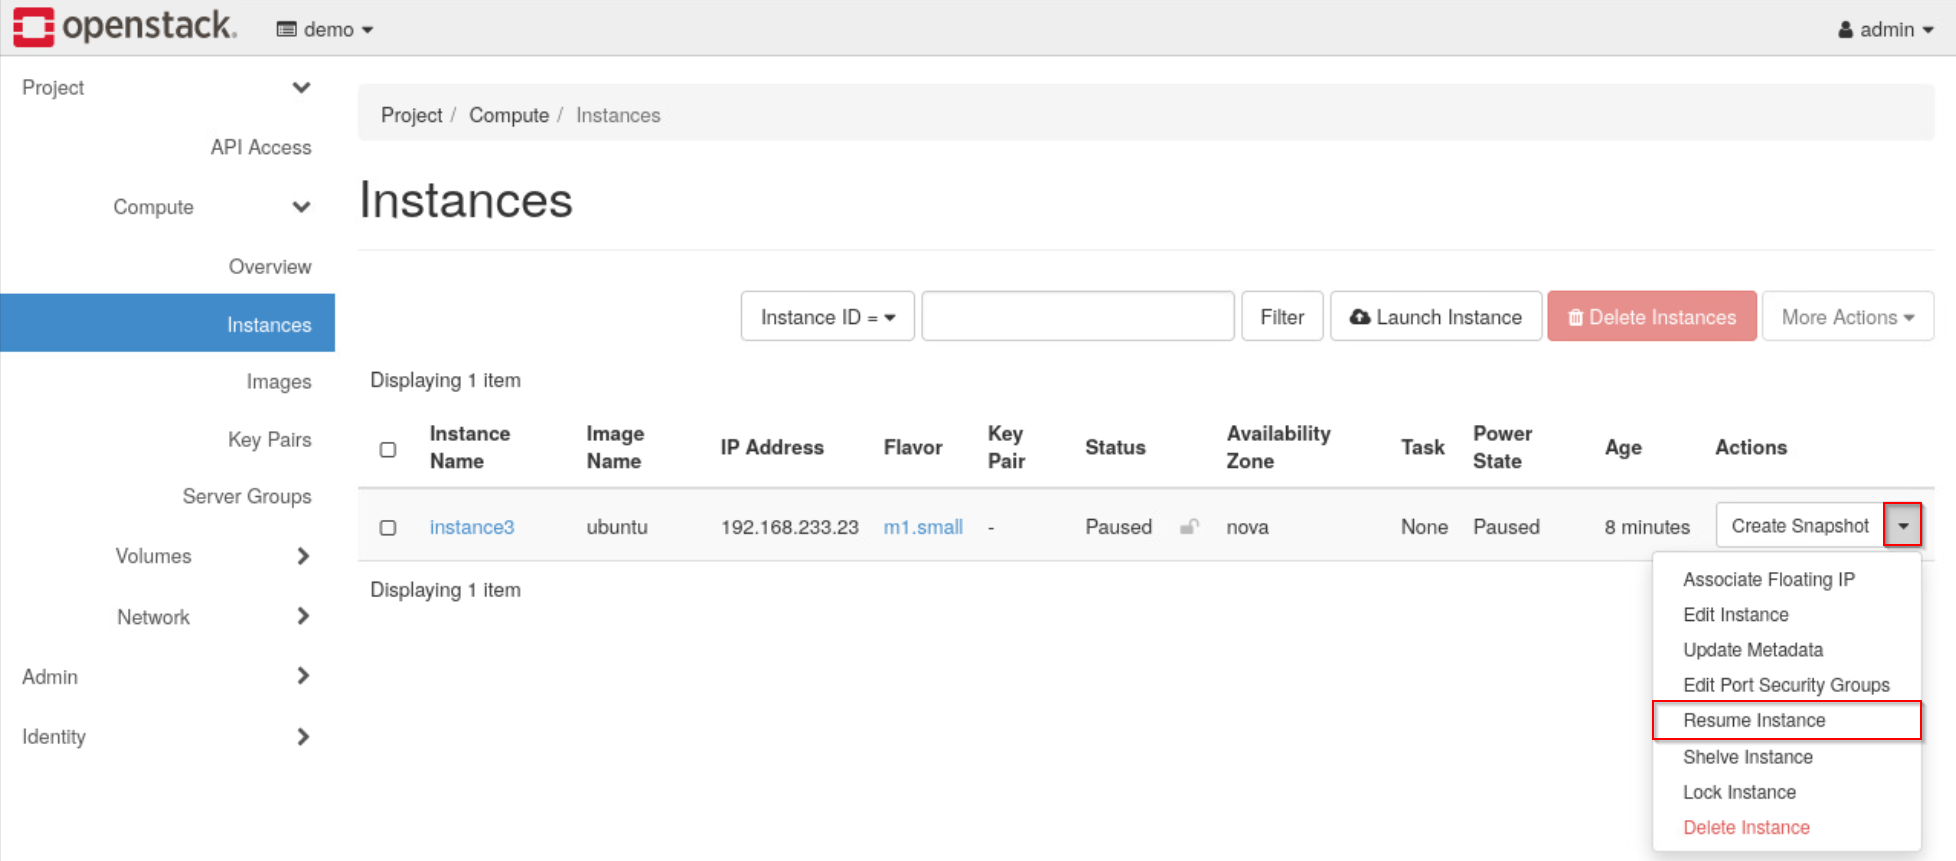
\includegraphics[width=\linewidth]{images/part3/step10.png}
        \end{center}
    \end{labstep}

    \begin{labstep}
        Click on \textbf{instance2} and select the \textbf{Console} tab to see that the ping replies have resumed.
        Press \textbf{Ctrl+C} to stop the \textbf{ping} process.

        \begin{center}
            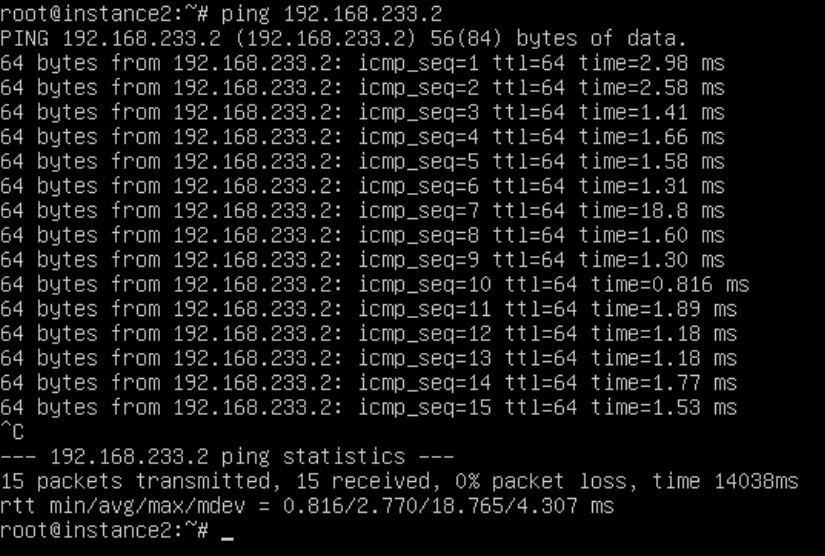
\includegraphics[width=\linewidth]{images/part3/step11.png}
        \end{center}
    \end{labstep}

    \begin{labstep}
        Shutting off or stopping an instance turns off the instance.
        The instance state and any data stored in the instance's RAM will be lost.
        Stopping an instance does not release its resources.
        To stop an instance, navigate to the \textbf{Instances} page.
        Click the dropdown next to \textbf{Create Snapshot} in the same row as \textbf{instance2} and click \textbf{Shut Off Instance}.

        \begin{center}
            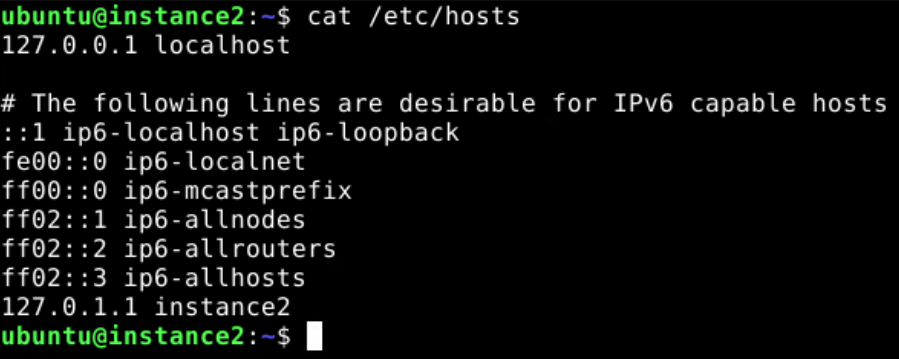
\includegraphics[width=\linewidth]{images/part3/step12.png}
        \end{center}
    \end{labstep}

    \begin{notebox}
        You may have to scroll down to find the option.
    \end{notebox}

    \begin{labstep}
        In the \textbf{Confirm Shut Off Instance} dialog, click \textbf{Shut Off Instance}.

        \begin{center}
            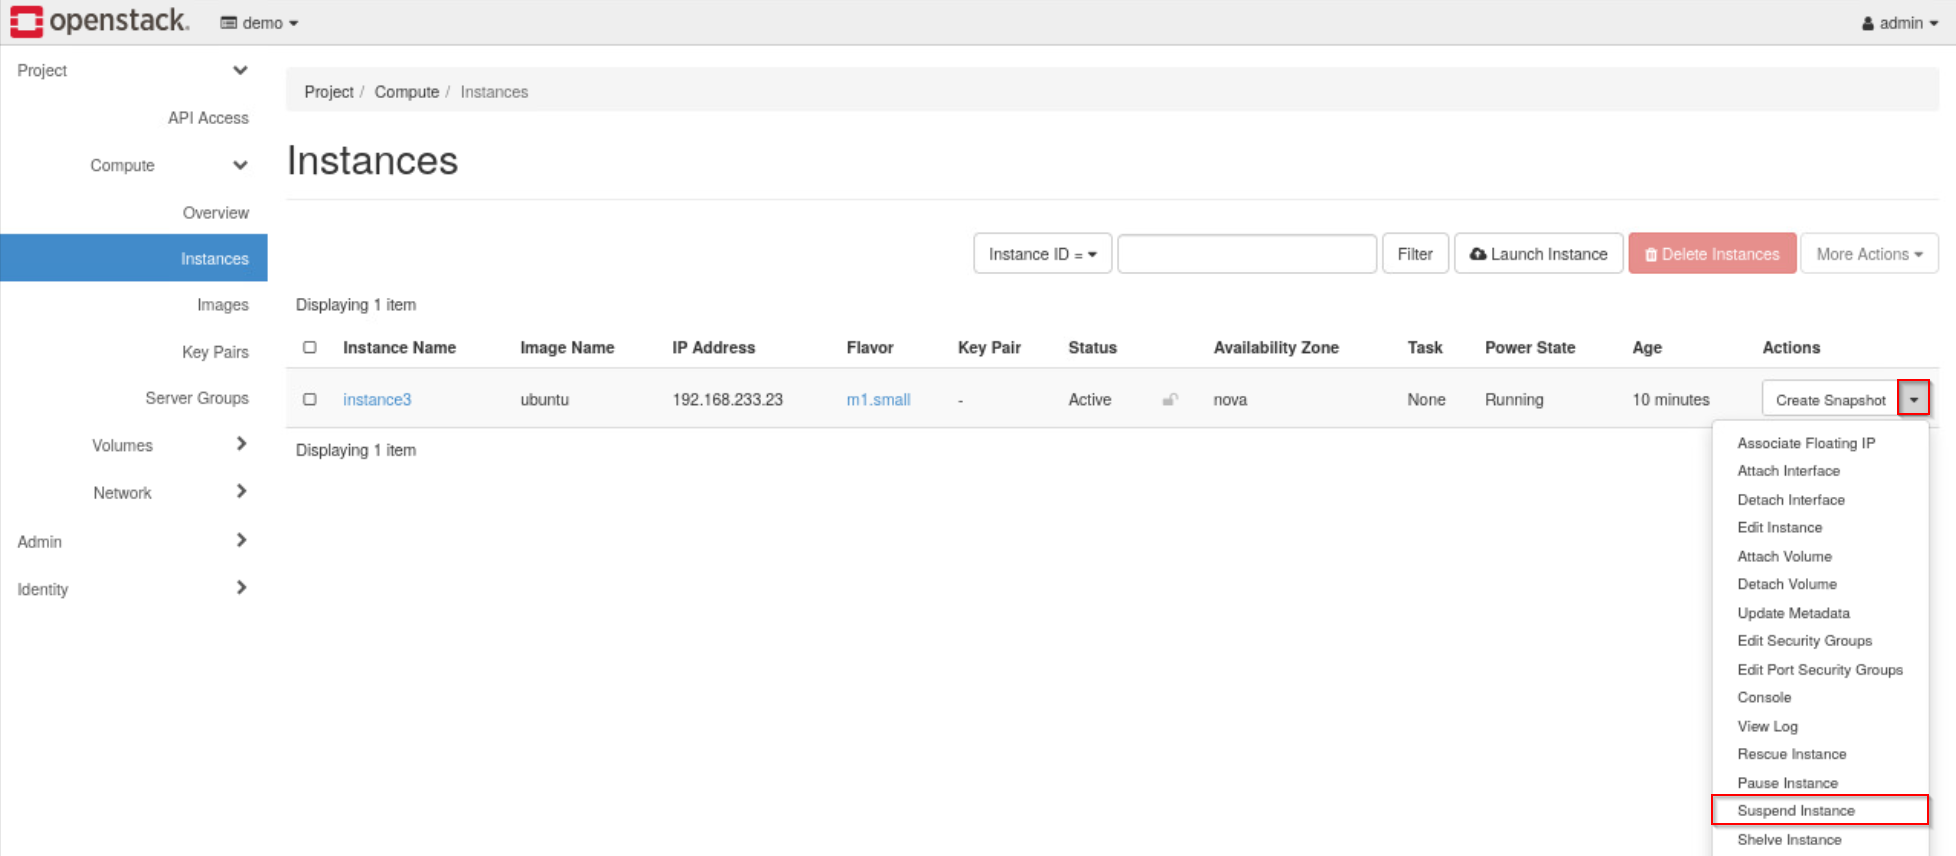
\includegraphics[width=\linewidth]{images/part3/step13.png}
        \end{center}
    \end{labstep}

    \begin{labstep}
        When the power state of the instance indicates that it is shut off, the \textbf{Create Snapshot} button will become \textbf{Start Instance}.
        Click this button to turn the instance back on.

        \begin{center}
            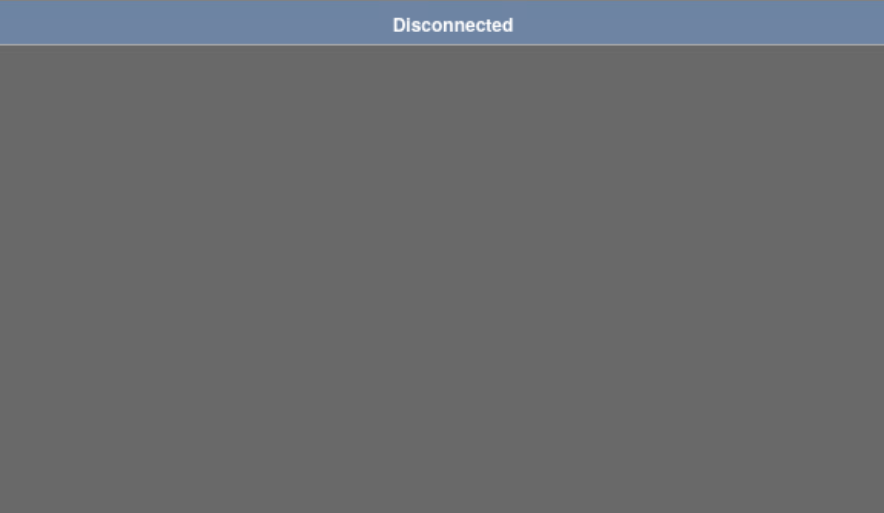
\includegraphics[width=\linewidth]{images/part3/step14.png}
        \end{center}
    \end{labstep}

    \begin{tipbox}
        In addition to shutting off an instance, an instance can also be soft or hard rebooted, or turned off and back on.
        A soft reboot allows the instance to perform a graceful shutdown, while hard rebooting an instance is analogous to pulling the power cord from a computer.
    \end{tipbox}

    \begin{labstep}
        Close the browser window and continue to the next task.
    \end{labstep}

\end{enumerate}

%%%%%%%%%%%
% Section 4
%%%%%%%%%%%
\section{Managing the Running State of an Instance with the OpenStack Unified CLI}\label{sec:managing_the_power_state_of_an_instance_cli}
In this task, you will repeat the steps from the previous task in the \textit{OpenStack Unified CLI}.

\begin{enumerate}
    \begin{labstep}
        If a terminal window is not already open, open one and source the keystone credentials for the \textbf{admin} user.
        \begin{lstlisting}
            ubuntu@workstation:~$ source ~/keystonerc-admin
        \end{lstlisting}

        \begin{center}
            \includegraphics[width=\linewidth]{images/part4/step1.png}
        \end{center}
    \end{labstep}

    \begin{labstep}
        Show the URL to the console of the instance.
        Right-click the URL and click \textbf{Open Link}.
        \begin{lstlisting}
            [ubuntu@workstation (keystone-admin)]:~$ openstack console url show instance2
        \end{lstlisting}

        \begin{center}
            \includegraphics[width=\linewidth]{images/part4/step2.png}
        \end{center}
    \end{labstep}

    \begin{labstep}
        Log in to \textbf{instance2} as \textbf{root} with the password \textbf{secret}.

        \begin{center}
            \includegraphics[width=\linewidth]{images/part4/step3.png}
        \end{center}
    \end{labstep}

    \begin{labstep}
        Continuously ping the DHCP server to see the effects of pausing an instance.
        \begin{lstlisting}
            root@instance2:~# ping 192.168.233.2
        \end{lstlisting}

        \begin{center}
            \includegraphics[width=\linewidth]{images/part4/step4.png}
        \end{center}
    \end{labstep}

    \begin{labstep}
        Focus back on the terminal window and pause the instance.
        \begin{lstlisting}
            [ubuntu@workstation (keystone-admin)]:~$ openstack server pause instance2
        \end{lstlisting}

        \begin{center}
            \includegraphics[width=\linewidth]{images/part4/step5.png}
        \end{center}
    \end{labstep}

    \begin{labstep}
        Now, view the browser window again to see that the instance is frozen and no more ping replies are appearing.

        \begin{center}
            \includegraphics[width=\linewidth]{images/part4/step6.png}
        \end{center}
    \end{labstep}

    \begin{labstep}
        Focus back on the terminal window and resume the instance
        \begin{lstlisting}
            [ubuntu@workstation (keystone-admin)]:~$ openstack server unpause instance2
        \end{lstlisting}

        \begin{center}
            \includegraphics[width=\linewidth]{images/part4/step7.png}
        \end{center}
    \end{labstep}

    \begin{labstep}
        View the browser window again to see that more ping replies are coming in.
        Press \textbf{Ctrl+C} to stop the \textbf{ping} process.

        \begin{center}
            \includegraphics[width=\linewidth]{images/part4/step8.png}
        \end{center}
    \end{labstep}

    \begin{labstep}
        Start the \textbf{ping} process again to view the effects of suspending an instance.
        \begin{lstlisting}
            root@instance2:~# ping 192.168.233.2
        \end{lstlisting}

        \begin{center}
            \includegraphics[width=\linewidth]{images/part4/step9.png}
        \end{center}
    \end{labstep}

    \begin{labstep}
        Focus back on the terminal window and suspend the instance.
        \begin{lstlisting}
            [ubuntu@workstation (keystone-admin)]:~$ openstack server suspend instance2
        \end{lstlisting}

        \begin{center}
            \includegraphics[width=\linewidth]{images/part4/step10.png}
        \end{center}
    \end{labstep}

    \begin{labstep}
        View the console again to see that the connection has been ended.
        When the instance is resumed, a new connection will be created, and this tab will still be unresponsive.
        Close the browser window.

        \begin{center}
            \includegraphics[width=\linewidth]{images/part4/step11.png}
        \end{center}
    \end{labstep}

    \begin{labstep}
        Focus back on the terminal window and resume the instance.
        \begin{lstlisting}
            [ubuntu@workstation (keystone-admin)]:~$ openstack server resume instance2
        \end{lstlisting}

        \begin{center}
            \includegraphics[width=\linewidth]{images/part4/step12.png}
        \end{center}
    \end{labstep}

    \begin{labstep}
        Show the URL to the console of the instance.
        Right-click the URL and click \textbf{Open Link}.
        \begin{lstlisting}
            [ubuntu@workstation (keystone-admin)]:~$ openstack console url show instance2
        \end{lstlisting}

        \begin{center}
            \includegraphics[width=\linewidth]{images/part4/step13.png}
        \end{center}
    \end{labstep}

    \begin{labstep}
        Log in to \textbf{instance2} as \textbf{root} with the password \textbf{secret}.

        \begin{center}
            \includegraphics[width=\linewidth]{images/part4/step14.png}
        \end{center}
    \end{labstep}

    \begin{labstep}
        Note that more ping replies are now coming in.
        Press \textbf{Ctrl+C} to stop the \textbf{instance}, and close the browser window.

        \begin{center}
            \includegraphics[width=\linewidth]{images/part4/step15.png}
        \end{center}
    \end{labstep}

    \begin{labstep}
        Focus back on the terminal window and confirm that \textbf{instance2} is listed as \textbf{ACTIVE}.
        \begin{lstlisting}
            [ubuntu@workstation (keystone-admin)]:~$ openstack server list \
            > --max-width 80
        \end{lstlisting}

        \begin{center}
            \includegraphics[width=\linewidth]{images/part4/step16.png}
        \end{center}
    \end{labstep}

    \begin{labstep}
        Stop the instance.
        \begin{lstlisting}
            [ubuntu@workstation (keystone-admin)]:~$ openstack server stop instance2
        \end{lstlisting}

        \begin{center}
            \includegraphics[width=\linewidth]{images/part4/step17.png}
        \end{center}
    \end{labstep}

    \begin{labstep}
        Verify that the status of \textbf{instance2} is \textbf{SHUTOFF}.
        \begin{lstlisting}
            [ubuntu@workstation (keystone-admin)]:~$ openstack server list \
            > --max-width 80
        \end{lstlisting}

        \begin{center}
            \includegraphics[width=\linewidth]{images/part4/step18.png}
        \end{center}
    \end{labstep}

    \begin{labstep}
        Power the instance back on.
        \begin{lstlisting}
            [ubuntu@workstation (keystone-admin)]:~$ openstack server start instance2
        \end{lstlisting}

        \begin{center}
            \includegraphics[width=\linewidth]{images/part4/step19.png}
        \end{center}
    \end{labstep}

    \begin{labstep}
        Verify that the status of \textbf{instance2} is \textbf{ACTIVE}.
        \begin{lstlisting}
            [ubuntu@workstation (keystone-admin)]:~$ openstack server list \
            > --max-width 80
        \end{lstlisting}

        \begin{center}
            \includegraphics[width=\linewidth]{images/part4/step20.png}
        \end{center}
    \end{labstep}

    \begin{labstep}
        The lab is now complete.
    \end{labstep}

\end{enumerate}
\end{document}
